%  LaTeX support: latex@mdpi.com 
%  For support, please attach all files needed for compiling as well as the log file, and specify your operating system, LaTeX version, and LaTeX editor.

%=================================================================
\documentclass[systems,article,accept,pdftex,moreauthors]{Definitions/mdpi} 
%\documentclass[preprints,article,submit,pdftex,moreauthors]{Definitions/mdpi} 
% For posting an early version of this manuscript as a preprint, you may use "preprints" as the journal. Changing "submit" to "accept" before posting will remove line numbers.


%=================================================================
% MDPI internal commands - do not modify
\firstpage{1} 
\makeatletter 
\setcounter{page}{\@firstpage} 
\makeatother
\pubvolume{1}
\issuenum{1}
\articlenumber{0}
\pubyear{2026}
\copyrightyear{2026}
\externaleditor{Firstname Lastname} % More than 1 editor, please add `` and '' before the last editor name
\datereceived{8 April 2026} 
\daterevised{1 May 2026} % Comment out if no revised date
\dateaccepted{3 May 2026} 
\datepublished{ } 
%\datecorrected{} % For corrected papers: "Corrected: XXX" date in the original paper.
%\dateretracted{} % For retracted papers: "Retracted: XXX" date in the original paper.
%\doinum{} % Used for some special journals, like molbank
%\pdfoutput=1 % Uncommented for upload to arXiv.org
%\CorrStatement{yes}  % For updates
%\longauthorlist{yes} % For many authors that exceed the left citation part
%\IsAssociation{yes} % For association journals



%=================================================================
% Add packages and commands here. The following packages are loaded in our class file: fontenc, inputenc, calc, indentfirst, fancyhdr, graphicx, epstopdf, lastpage, ifthen, float, amsmath, amssymb, lineno, setspace, enumitem, mathpazo, booktabs, titlesec, etoolbox, tabto, xcolor, colortbl, soul, multirow, microtype, tikz, totcount, changepage, attrib, upgreek, array, tabularx, pbox, ragged2e, tocloft, marginnote, marginfix, enotez, amsthm, natbib, hyperref, cleveref, scrextend, url, geometry, newfloat, caption, draftwatermark, seqsplit
% cleveref: load \crefname definitions after \begin{document}

%=================================================================
% Please use the following mathematics environments: Theorem, Lemma, Corollary, Proposition, Characterization, Property, Problem, Example, ExamplesandDefinitions, Hypothesis, Remark, Definition, Notation, Assumption
%% For proofs, please use the proof environment (the amsthm package is loaded by the MDPI class).

%=================================================================
% Full title of the paper (Capitalized)
\Title{Operational Data Foundation Framework for Smart Manufacturing in SMEs: Field Implementation and Evaluation}

% Author Orchid ID: enter ID or remove command
\newcommand{\orcidauthorA}{0009-0003-4190-193X}
\newcommand{\orcidauthorB}{0000-0001-6553-7448}

% Authors, for the paper (add full first names)
\Author{Yoonseok Kang $^{1}$\orcidA{} and Dongchul Park $^{2,}$*\orcidB{}}

%\longauthorlist{yes}

% MDPI internal command: Authors, for metadata in PDF
\AuthorNames{Yoonseok Kang and Dongchul Park}

%\longauthorlist{yes}

% Affiliations / Addresses (Add [1] after \address if there is only one affiliation.)
\address{%
$^{1}$ \quad Department of Convergence Security, Chung-Ang University, Seoul 06974, Republic of Korea; kangcl1609@cau.ac.kr\\
$^{2}$ \quad Department of Industrial Security, Chung-Ang University, Seoul 06974, Republic of Korea; dongchul@cau.ac.kr
}

% Contact information of the corresponding author
\corres{Correspondence: dongchul@cau.ac.kr}
%; Tel.: (optional; include country code; if there are multiple corresponding authors, add author initials) +xx-xxxx-xxx-xxxx (F.L.)}




% Abstract (Do not insert blank lines, i.e. \\) 
\abstract{
Smart manufacturing depends on operational data that remain continuous, interpretable, and reusable in practice. In constrained small- and medium-sized enterprise (SME) factories, however, the main bottleneck often lies not in later-stage analytics or AI applications but in securing an operationally viable data foundation under real deployment conditions. A lifecycle-based analysis of smart manufacturing data pipelines, together with recurrent SME deployment constraints identified in prior studies, led this study to derive six recurring operational risks. On this basis, this study proposes an \emph{\highlighting{Operational Data Foundation Framework} %MDPI: Please confirm if the italics are necessary; if not, please remove them. The following highlights are the same.
} structured around core requirements of continuity, governance, diagnosability, operability, reprocessability, and evolvability. These requirements are further articulated through design principles and assessable operational invariants. The framework was instantiated in a real SME factory, where heterogeneous field sources were integrated into a coherent operational data foundation for smart manufacturing through constrained communication paths, durable edge-side capture, cloud-side stream processing, controlled data normalization, and monitoring and alerting functions. Requirement-based evidence from the field implementation showed that the system preserved stable semantics across the pipeline, made failures traceable to specific lifecycle segments, preserved historical records for later reprocessing, and remained manageable under constrained deployment conditions. A representative field case further demonstrated the framework's practical value: severe communication instability was diagnosed through lifecycle-segment discrepancy analysis and improved from approximately 33\% to 95\% packet reception after targeted intervention. This study contributes a field-grounded and assessable design logic for operational data foundations, with field evidence from a single food manufacturing SME supporting its feasibility and operational relevance.
}

% Keywords
\keyword{smart manufacturing; SME digitalization; operational data foundation; \linebreak industrial data infrastructure; data governance} 

%(List three to ten pertinent keywords specific to the article; yet reasonably common within the subject discipline.)

% The fields PACS, MSC, and JEL may be left empty or commented out if not applicable
%\PACS{J0101}
%\MSC{}
%\JEL{}






%%%%%%%%%%%%%%%%%%%%%%%%%%%%%%%%%%%%%%%%%%
\begin{document}

%%%%%%%%%%%%%%%%%%%%%%%%%%%%%%%%%%%%%%%%%%
%%%%%%%%%%%%%%%%%%%%%%%%%%%%%%%%%%%%%%%%%%
\section{Introduction}
\label{sec:introduction}

Smart manufacturing is transforming manufacturing from a production environment centered primarily on physical equipment and isolated processes into a connected operational system built on continuous data flows \cite{song2025smart,tao2018datadriven}. Across the factory, sensing, communication, computation, and decision making are becoming increasingly integrated through technologies such as the Internet of Things (IoT), cyber--physical systems (CPS), artificial intelligence and machine learning (AI/ML), real-time monitoring, predictive maintenance, and digital twins \cite{tao2017digital,ding2019digital,nguyen2025aidriven}. Manufacturing systems should therefore be understood not only as physical production arrangements, but also as data-mediated operational systems \cite{cerquitelli2021manufacturing}.

In smart manufacturing, data no longer serve merely as records of what has already happened. They have become a core operational resource that supports visibility, traceability, quality control, maintenance, and data-driven decision making \cite{ren2019bigdata,tao2018datadriven}. As a result, the practical progress  of smart manufacturing increasingly depends on whether operational data can be captured, interpreted, and reused in a stable and sustained manner \cite{bernstein2018contextualising}.

Higher-level capabilities such as predictive analytics, digital twins, and AI-driven optimization do not become operational simply by being introduced. They depend on an underlying data layer that can continuously capture field conditions, preserve meaning across system boundaries, and support downstream reuse \cite{walton2024unified,zaborowski2024role}. The central issue, therefore, is not only what manufacturing systems can do intelligently, but what kind of data foundation must first be maintained to make such intelligence workable in practice.

The value of manufacturing data does not lie in data generation alone. It is realized across an end-to-end flow in which field data are acquired, transmitted, transformed, stored, and reused downstream \cite{ismail2019manufacturing,raptis2019data}. Manufacturing data problems should therefore be understood not as isolated database or interface issues, but as lifecycle-wide operational systems problems \cite{hedberg2017lift}. This challenge becomes more acute in industrial environments, where heterogeneous devices, protocols, timestamps, machine states, manual records, and fragmented platforms coexist \cite{zeid2019interoperability,pereira2021towards}. Under such conditions, missingness, duplication, delay, semantic inconsistency, and timestamp ambiguity directly weaken traceability, operational visibility, and decision quality \cite{morris2020foundations,foidl2024pipeline}.

What is required, therefore, is not merely an ingestion infrastructure, but an operational layer that can preserve continuity, governed semantics, durable persistence, observability, and downstream reusability across that lifecycle \cite{morris2020foundations,davis2020cyberinfrastructure}. In this study, we refer to this layer as the \emph{operational data foundation}. Rather than functioning as a simple conduit for data movement, it stabilizes heterogeneous field data and makes them dependable for sustained operational and analytical use. As illustrated in Figure~\ref{fig:odf_position}, this layer occupies the space between heterogeneous operational data sources and higher-level operational and analytical applications.

\begin{figure}[H]
    %\centering
    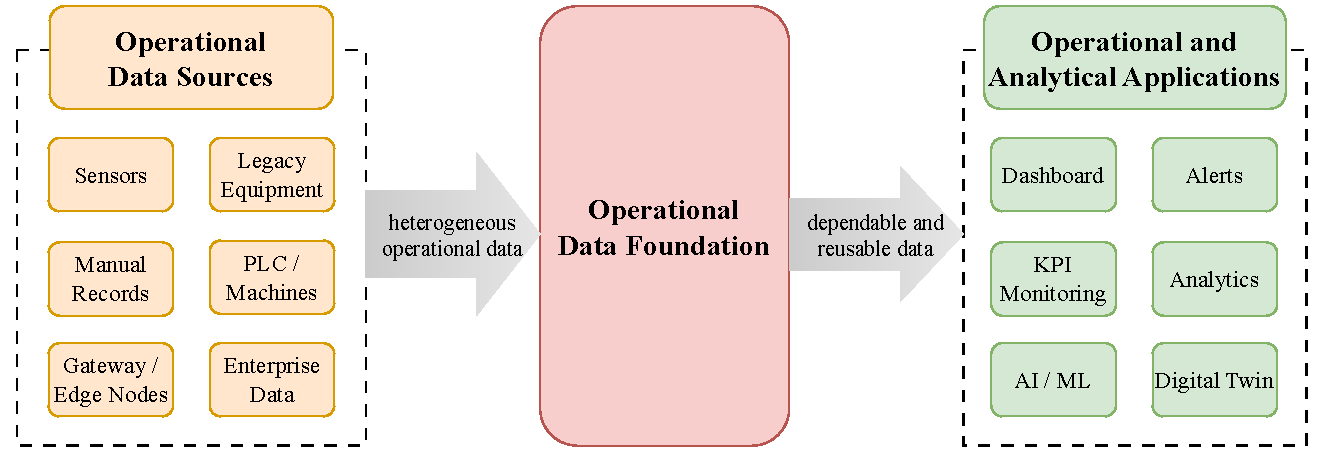
\includegraphics[width=\textwidth]{figures/Data_Foundation.pdf}
    \caption{Position of the operational data foundation in a digitalized manufacturing system.}
    \label{fig:odf_position}
\end{figure}

Although dependable manufacturing data systems are difficult to build in general, their practical design requirements become most visible in constrained SME \mbox{factories \cite{mittal2018maturity,krishnan2024challenges}}. These environments rarely provide the conditions often assumed in digitally mature smart-manufacturing settings, such as standardized interfaces, stable internal connectivity, dedicated technical support, and integrated data infrastructure \cite{mittal2020adoption,ghobakhloo2019adoption}. Instead, they are more commonly characterized by legacy equipment, fragmented systems, mixed communication technologies, manual records, limited technical staffing, and strong cost sensitivity \cite{alqoud2022legacy,huang2025barriers}. SME factories should therefore be understood not merely as smaller plants, but as critical design settings in which the practical assumptions of smart manufacturing data systems are tested most directly \cite{krishnan2024challenges}.

In such environments, the main bottleneck of digitalization does not lie simply in deploying more sensors, collecting more data, or adding downstream applications. Rather, it lies in whether operational data can be captured with continuity, stabilized with interpretable meaning, and sustained as a usable resource despite fragmentation, instability, and limited operational slack. The central difficulty in SME manufacturing is therefore not merely data scarcity, but the fragility of the operational data lifecycle through which field data must become dependable for ongoing operational use \cite{kumar2025digitalization,narwane2022examining,morris2020foundations}.

This implies that the primary bottleneck of smart manufacturing in constrained SME factories lies not in downstream intelligence itself, but in establishing an operationally viable data foundation. Accordingly, this study examines how an operational data foundation should be designed, and what it must guarantee, in order to make smart manufacturing practically viable in constrained SME factories.

Existing research has approached manufacturing data systems from several complementary directions. Smart manufacturing studies have mainly focused on higher-level applications such as real-time monitoring, predictive maintenance, digital twins, and adaptive production support \cite{song2025smart,tao2017digital,nguyen2025aidriven}. Research on industrial data infrastructures has examined pipelines, integration architectures, edge--cloud coordination, governance, and data \mbox{quality \cite{ismail2019manufacturing,raptis2019data,morris2020foundations}}. Lifecycle-oriented work has emphasized cross-stage linkage, traceability, contextual continuity, and the preservation of reusable records \cite{bernstein2018contextualising,hedberg2017lift,abdelaty2024conceptualizing,zhang2024digitalthread}. Meanwhile, studies on SME digitalization have clarified the realities of constrained deployment, including legacy equipment, fragmented systems, limited staffing, and cost sensitivity \cite{mittal2020adoption,ghobakhloo2019adoption,krishnan2024challenges,huang2025barriers}.

However, these contributions remain only partially integrated when the problem is viewed from the standpoint of operational viability under constrained deployment conditions. Prior work has often examined applications, architectural components, lifecycle properties, or SME constraints separately, rather than formalizing what a manufacturing data foundation itself must guarantee in order to remain usable in practice. As a result, there is still limited systems-level understanding of how such guarantees should be defined, structured, and assessed in constrained SME manufacturing environments.

To address this gap, this study focuses on the foundational layer presupposed by smart manufacturing applications and formalizes it in terms of operational requirements, design principles, and assessable invariants. More specifically, it develops an \emph{\hl{Operational Data Foundation Framework}} for constrained SME factories and examines it not only conceptually, but also through field implementation and operational evidence from a real SME \mbox{manufacturing deployment}.

On this basis, the study is guided by the following research questions:

\begin{itemize}
    \item \textbf{\hl{RQ1.} %MDPI: Please confirm if the bold formatting is necessary; if not, please remove it. The following highlights are the same.
} What operational risks emerge when smart manufacturing data pipelines are deployed under constrained SME factory conditions?
    \item \textbf{\hl{RQ2.}} What core requirements must an operational data foundation satisfy under such conditions, and how can these requirements be formalized into design principles and operational invariants?
    \item \textbf{\hl{RQ3.}} How can the proposed framework be instantiated in a real SME manufacturing setting, and how can its practical value be evaluated through field evidence?
\end{itemize}

To address these questions, the study proceeds in four steps. First, it establishes a general lifecycle model of smart manufacturing data pipelines as an analytical reference. It then analyzes how recurrent constraints identified in prior SME research act across that lifecycle and derives six operational risks that undermine practical viability. On that basis, it formalizes the Operational Data Foundation Framework by translating those risks into core requirements, design principles, and operational invariants. Finally, it instantiates the framework through field implementation in a real SME manufacturing setting and evaluates its practical value through requirement-based evidence and representative field observations.

The primary contributions of this research are as follows:

\begin{enumerate}
    \item Reframing the practical bottleneck of smart manufacturing in constrained SME factories as an operational data foundation problem.
    \item Deriving the core operational risks that emerge when a general manufacturing data lifecycle is exposed to constrained SME factory conditions.
    \item Formalizing the Operational Data Foundation Framework in terms of core requirements, design principles, and operational invariants.
    \item Demonstrating the framework's feasibility and field-grounded operational relevance through real-world implementation in a single food manufacturing SME.
\end{enumerate}

The remainder of this paper is organized as follows. Section~\ref{sec:related_work} reviews the related literature. Section~\ref{sec:problem_analysis} analyzes the general data pipeline lifecycle, SME-specific constraints, and the resulting operational risks. Section~\ref{sec:odff} presents the proposed Operational Data Foundation Framework. Section~\ref{sec:field_implementation} describes the field implementation in an SME manufacturing setting. Section~\ref{sec:framework_evaluation} evaluates the framework using requirement-based evidence and field observations. Finally, Section~\ref{sec:conclusion} concludes the paper.


%%%%%%%%%%%%%%%%%%%%%%%%%%%%%%%%%%%%%%%%%%
%%%%%%%%%%%%%%%%%%%%%%%%%%%%%%%%%%%%%%%%%%
\section{Related Work}
\label{sec:related_work}

%%%%%%%%%%%%%%%%%%%%%%%%%%%%%%%%%%%%%%%%%%
\subsection{Smart Manufacturing Applications}
\label{sec:smart_manufacturing_applications}

Smart manufacturing research has developed primarily around higher-level applications and intelligent capabilities, including industrial IoT, cyber--physical systems, digital twins, real-time monitoring, predictive maintenance, and AI/ML-enabled decision \mbox{making \cite{rozhok2026advanced, bueno2020smart, cinar2020digital, atalay2022digital}}. Across these streams, the dominant aim has been to make manufacturing systems more connected, adaptive, and data-driven through enhanced visibility, prediction, and control \cite{rozhok2026advanced, bueno2020smart, song2025smart}.

Recent studies have extended this application-oriented stream toward more scalable and distributed forms of smart manufacturing. Digital twin architectures have been combined with Edge AI, federated learning, and physics-based co-simulation for distributed real-time decision making \cite{padmavathi2025digital}, while other work has integrated digital twins, ontology-based modeling, optimization, and automated simulation for dynamic line reconfiguration under disturbances \cite{fu2025digital}.

Despite their diversity, these applications share a common prerequisite: continuous or near-real-time operational data from the shop floor \cite{nguyen2025aidriven, tao2017digital, ding2019digital}. Studies on digital twins and real-time manufacturing intelligence repeatedly show that higher-level functions depend on data that are accurate, timely, and interpretable, and that remain aligned with physical system states \cite{nguyen2025aidriven, ojstersek2023optimizing, qamsane2019digital}. Yet this literature is generally more explicit about what smart manufacturing applications can optimize, predict, or automate than about what kind of data basis must be sustained for those functions to remain operationally viable in \mbox{practice \cite{rozhok2026advanced, ciano2021digital, nguyen2025aidriven}}.

%%%%%%%%%%%%%%%%%%%%%%%%%%%%%%%%%%%%%%%%%%
\subsection{Industrial Data Infrastructures}
\label{sec:industrial_data_infrastructures}

A substantial body of research has examined the industrial data basis through manufacturing data pipelines, integration architectures, industrial data management systems, and edge--cloud infrastructures \cite{ismail2019manufacturing, raptis2019data, saqlain2019framework}. This literature makes clear that manufacturing data handling is not merely a storage problem, but a multi-layer systems problem spanning acquisition, communication, processing, storage, and downstream delivery across heterogeneous sources \cite{ismail2019manufacturing, odonovan2015industrial}.

Within this stream, two themes are especially prominent. First, many studies address heterogeneous integration and interoperability across legacy equipment, devices, protocols, platforms, and enterprise systems \cite{zeid2019interoperability, pereira2021towards, modoni2017enhancing}. Second, related work has emphasized semantics, context, and governance, arguing that industrial data must remain interpretable, trustworthy, and reusable rather than merely transferable \cite{hildebrandt2020ontology, morris2020foundations, westermann2022accessing}. These contributions have significantly advanced understanding of how industrial data infrastructures can be connected, organized, and managed. However, they remain more focused on components, architectures, and enabling techniques than on explicitly formalizing what such infrastructures must guarantee as an operational foundation under deployment \mbox{constraints \cite{ismail2019manufacturing, raptis2019data, morris2020foundations}}.

This infrastructure-oriented view also aligns with systems engineering and systems thinking perspectives. In constrained SME manufacturing, industrial data infrastructure is not merely a set of technical components, but a socio-technical system in which field devices, communication paths, edge nodes, storage layers, data contracts, dashboards, and human operators interact across technical and organizational boundaries \cite{Panchal2024,Rebentisch2022}. From this perspective, data loss, semantic inconsistency, weak observability, and maintenance burden can be understood not only as local technical defects, but also as effects of interactions among heterogeneous components, operational routines, and deployment constraints. Recent smart manufacturing pipeline research similarly highlights legacy integration, lightweight deployment, and heterogeneous data coordination as continuing infrastructure challenges \cite{Ceselli2025}. This systems-oriented interpretation supports the position of this study: an operational data foundation should be formalized not only as a data pipeline architecture, but as lifecycle-wide guarantees that preserve coherence across distributed technical and operational elements.

%%%%%%%%%%%%%%%%%%%%%%%%%%%%%%%%%%%%%%%%%%
\subsection{Lifecycle Connectivity}
\label{sec:lifecycle_connectivity}

Another important line of research treats manufacturing data not as stage-local records, but as lifecycle-wide resources. From this perspective, the value of manufacturing data depends on whether information can remain linked, contextualized, and reusable across design, production, inspection, operation, maintenance, and end-of-life stages \cite{ren2019bigdata, tao2018datadriven, bernstein2018contextualising, hedberg2017lift}. This perspective shifts attention away from isolated data handling and toward continuity of meaning and usability across lifecycle transitions.

The concept of the digital thread has become the clearest expression of this perspective. Recent reviews and implementation studies define the digital thread as a means of linking information across heterogeneous lifecycle artifacts and stages so that traceability, cross-stage visibility, and lifecycle-wide reuse become possible beyond fragmented system silos \cite{abdelaty2024conceptualizing, zhang2024digitalthread, bianchini2024digitalthread, hedberg2020graphs}. Related studies on contextualization, standards-based linkage, and knowledge-graph integration likewise show that lifecycle usefulness depends not merely on storing records, but on preserving associativity, context, and interpretability for later reuse \cite{kwon2020enriching, schmidt2018flow, monnier2022methodology}. At the same time, this literature has focused mainly on linkage and traceability, with relatively less explicit discussion of how such continuity and reuse can be sustained operationally under constrained deployment conditions.

%%%%%%%%%%%%%%%%%%%%%%%%%%%%%%%%%%%%%%%%%%
\subsection{SME Deployment}
\label{sec:sme_deployment}

The SME literature makes those deployment constraints explicit. Studies on smart manufacturing adoption in SMEs consistently show that these environments differ substantially from idealized smart factory assumptions: legacy equipment, fragmented systems, uneven interfaces, limited digital infrastructure, restricted investment capacity, and uneven technical expertise are common \cite{mittal2018maturity, mittal2020adoption, ghobakhloo2019adoption, krishnan2024challenges}. In this sense, SMEs should not be viewed simply as smaller versions of large factories, but as constrained deployment settings in which the assumptions of digitally mature architectures are most directly challenged.

These constraints are both technical and operational. Brownfield dependence often forces SMEs to rely on retrofitting, add-on sensing, gateway-based integration, and low-cost connectivity rather than wholesale replacement \cite{alqoud2022legacy, etz2020retrofit, tran2022retrofitting, park2019opcua}. At the same time, recurring barriers include limited staffing, weak digital skills, uncertain return on investment, high implementation cost, and maintenance burden \cite{huang2025barriers, narwane2022examining, kumar2025digitalization, hulla2021towards}. Accordingly, SME-oriented studies increasingly advocate phased, modular, and capability-building adoption \mbox{paths \cite{chavez2020capability, krishnan2024challenges, banerjee2024lowcost}}. Taken together, these studies show that the unresolved problem is not how to deploy smart manufacturing applications, infrastructure components, or lifecycle linkage mechanisms, but how to sustain a data foundation that remains operationally viable under constrained real-world conditions.

%%%%%%%%%%%%%%%%%%%%%%%%%%%%%%%%%%%%%%%%%%
%%%%%%%%%%%%%%%%%%%%%%%%%%%%%%%%%%%%%%%%%%
\section{Problem Analysis}
\label{sec:problem_analysis}

This section analyzes the data basis of smart manufacturing as an operational pipeline and examines how constrained SME factory conditions introduce structural fragility across that pipeline. Rather than merely describing deployment difficulty, it identifies how lifecycle-wide constraints converge into a small set of recurring operational risks. In this way, the section defines the problem structure of operational data foundations under constrained deployment conditions.

%%%%%%%%%%%%%%%%%%%%%%%%%%%%%%%%%%%%%%%%%%
\subsection{General Data Pipeline Lifecycle}
\label{sec:data_lifecycle}


A common analytical reference is needed before constrained SME conditions and their resulting risks can be examined in a structured manner. In smart manufacturing, data do not become operationally useful at the moment of generation alone. Their practical value emerges only through a broader path in which field observations are accepted into a pipeline, transferred across infrastructure layers, transformed into usable forms, preserved, and connected to downstream operational use \cite{ismail2019manufacturing,raptis2019data}. For this reason, this study adopts a \emph{\hl{general data pipeline lifecycle}} as an analytical frame for problem interpretation rather than as a normative system architecture.

The lifecycle used in this study is shown in Figure~\ref{fig:data_lifecycle}. It is adapted from generic data pipeline literature, which treats data systems as multi-stage processing structures characterized by recurring issues related to ingestion, integration, cleaning, transformation, loading, and pipeline-wide quality control \cite{foidl2024pipeline}. In the smart manufacturing context, this general view is organized as follows:

\begin{itemize}
    \item \textbf{\hl{Data sources:}} %MDPI: Please confirm if the bold formatting is necessary; if not, please remove it. The following highlights are the same.
    The points at which operational data originate, including sensors, equipment states, manual records, and external systems.
    \item \textbf{\hl{Data ingestion:}} The intake of source data into the pipeline.
    \item \textbf{\hl{Data transmission:}} The movement of acquired data across gateway, edge, server, or cloud boundaries toward the next processing point.
    \item \textbf{\hl{Data preprocessing:}} The cleaning, decoding, normalization, mapping, and transformation required to make raw inputs usable downstream.
    \item \textbf{\hl{Data loading:}} The controlled insertion of processed records into the target operational layer or storage boundary.
    \item \textbf{\hl{Data storage:}} The durable preservation of records for later access, recovery, reinterpretation, and reuse.
    \item \textbf{\hl{Data sinks:}} The downstream endpoints that consume stored data, including dashboards, alerts, reporting, analytics, and decision support.
\end{itemize}

This lifecycle is analytically useful because it makes visible the full path through which manufacturing data become operationally usable. At the same time, it does not by itself provide a design answer. It describes how data move, but not what must be preserved for the lifecycle to remain operationally viable under constrained conditions. It is therefore used in this study as an analytical reference for the constraint and risk analysis that follows.


\begin{figure}[H]
    %\centering
    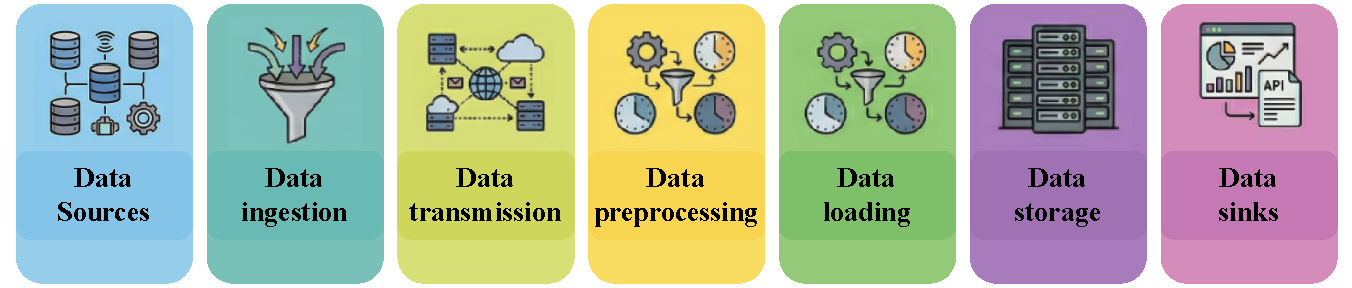
\includegraphics[width=1\linewidth]{figures/3-1_Data_Lifecycle.pdf}
    \caption{General data pipeline lifecycle in smart manufacturing.}
    \label{fig:data_lifecycle}
\end{figure}

%%%%%%%%%%%%%%%%%%%%%%%%%%%%%%%%%%%%%%%%%%
\subsection{SME Constraints}
\label{sec:sme_constraints}


Constrained SME factories should not be treated simply as smaller versions of digitally mature plants. Prior research shows that their starting conditions are structurally different: legacy equipment, fragmented systems, uneven interfaces, restricted digital infrastructure, limited internal expertise, and strong investment sensitivity are common, whereas standardized connectivity and unified data access are often absent \cite{mittal2018maturity, mittal2020adoption, ghobakhloo2019adoption, krishnan2024challenges, rauch2019requirements}. SME constraints are therefore better understood not as isolated implementation difficulties, but as recurring design conditions that act across the general data pipeline lifecycle. Figure~\ref{fig:3-2_data_lifecycle} highlights this point by showing how the major constraint types propagate across source capture, transfer, transformation, storage, and downstream use, rather than remaining confined to a \mbox{single stage}.

Heterogeneity begins at the source side. In SME factories, brownfield machinery, retrofit-based extension, add-on sensing, and gateway-mediated access are common, so inconsistency is already present at the level of data sources and ingestion rather than arising only later during integration \cite{alqoud2022legacy, etz2020retrofit, tran2022retrofitting, park2019opcua}. The challenge is not merely to collect values, but to incorporate diverse formats, units, reporting intervals, and source identities into a coherent operational structure. Source-side variability is therefore not a peripheral inconvenience, but the starting condition from which later coordination and interpretation problems emerge.

Transmission is often fragile in constrained SME deployments. Field data may depend on low-cost wireless communication, battery-powered sensing, and gateway- or edge-dependent relay paths rather than on stable plant-wide infrastructure \cite{gao2019connectivity, noor2023wireless, hawkridge2019tying}. The ingestion--transmission path therefore becomes a distinct surface of instability. What matters operationally is not simply whether a value was observed once, but whether the record can remain sufficiently continuous and recoverable despite interruption, delay, and \mbox{relay dependence}.

Operational meaning must remain stable across the pipeline. Manufacturing data are operationally usable only when source identity, metric semantics, unit interpretation, and time semantics remain controlled across preprocessing, loading, and storage. Yet constrained environments frequently rely on heterogeneous preprocessing logic, ad hoc mappings, incomplete context, and weak contract discipline, making semantic drift and traceability loss structurally likely \cite{pereira2021towards, nagorny2020rami, hildebrandt2020ontology, westermann2022accessing, morris2020foundations}. Once such instability becomes embedded in stored records, downstream analytics and dashboards may continue to function while resting on an increasingly fragile semantic basis.

These technical difficulties are intensified by operational realities. SME studies repeatedly report limited staffing, uneven digital skills, manual troubleshooting, high maintenance burden, and weak strategic capacity \cite{huang2025barriers, kumar2025digitalization, hulla2021towards, nasirinejad2024maintenance}. At the same time, SME digitalization rarely proceeds as a one-shot transformation; instead, it unfolds through phased rollout, retrofit-based extension, KPI revision, and incremental onboarding of new sources and processes \cite{chavez2020capability, doyle2019steps, mcfarlane2022digitalisation, banerjee2024lowcost}. As a result, the practical challenge is not only whether a system can be built, but whether it can remain diagnosable, manageable, and adaptable as requirements evolve.

Taken together, these observations show that the core problem in constrained SME factories is not simply that deployment is difficult. Rather, the assumptions of the general data pipeline lifecycle are systematically destabilized across the lifecycle itself: records may lose continuity, meanings may drift, failures may become difficult to localize, operational burden may increase, historical data may lose replay value, and later extension may require disproportionate rework. The next subsection translates these recurring forms of fragility into the language of operational risk.


\begin{figure}[H]
   % \centering
    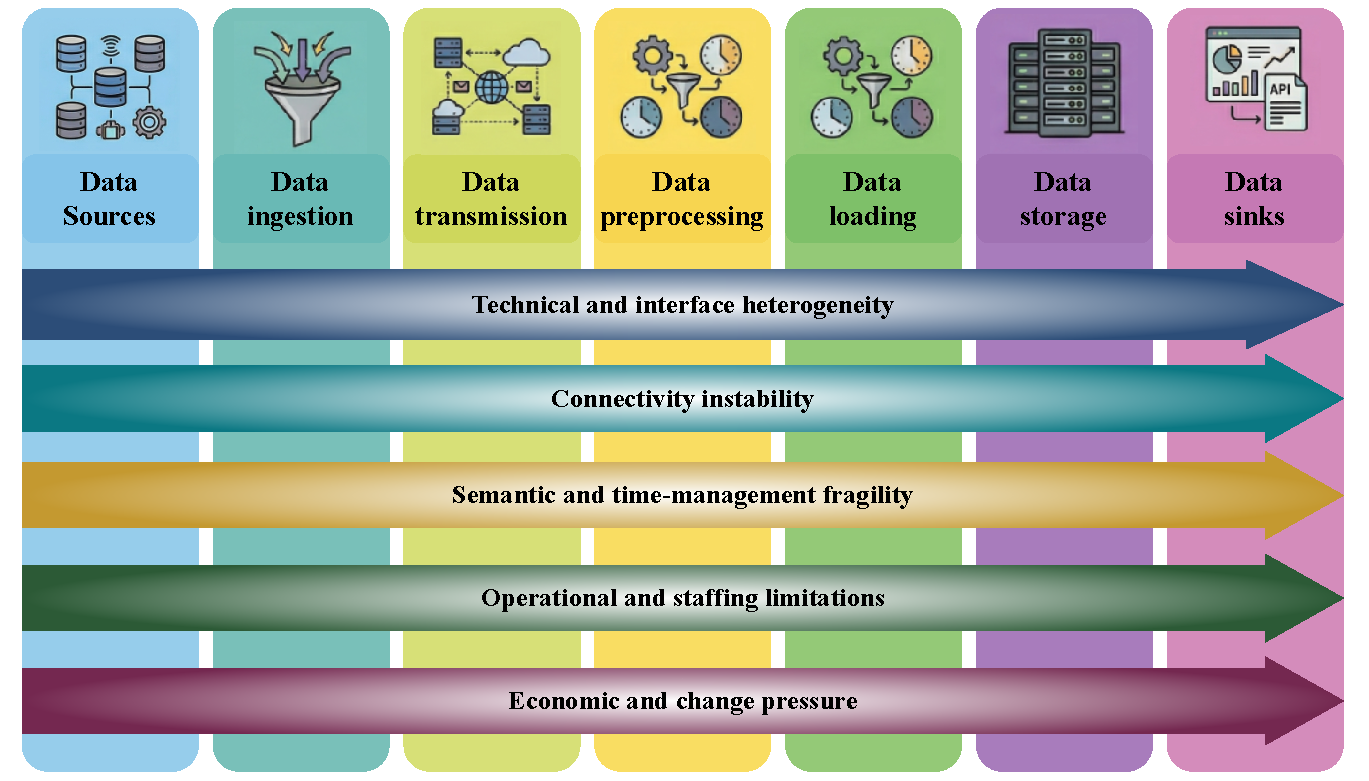
\includegraphics[width=1\linewidth]{figures/3-2_Data_Lifecycle.pdf}
    \caption{\hl{SME} %MDPI: Please confirm whether an explanation of the arrow and different colors needs to be added to the figure caption.
 constraints across the general data pipeline lifecycle.}
    \label{fig:3-2_data_lifecycle}
\end{figure}


%%%%%%%%%%%%%%%%%%%%%%%%%%%%%%%%%%%%%%%%%%
\subsection{Operational Risks}
\label{sec:operational_risks}

The SME constraints discussed above do not remain isolated deployment difficulties. When mapped onto the general data pipeline lifecycle, they appear as recurring operational risks that determine whether manufacturing data can remain usable in practice. The issue, therefore, is not only how data move through the pipeline, but also what must be preserved for the resulting record to remain dependable under constrained real-world conditions.

\begin{itemize}[leftmargin=1.5em]
    \item[\textbf{\hl{RSK1.}}] \textbf{\hl{Continuity risk:}} %MDPI: Please confirm if the list format and bold should be kept. The following highlights are the same.
    Operational records may become interrupted, fragmented, or partially lost as data move from source capture to storage. In constrained manufacturing settings, the essential requirement is not one-time collection success, but the preservation of a gap-minimized and recoverable record despite source instability, transmission disruption, or delayed recovery.

    \item[\textbf{\hl{RSK2.}}] \textbf{\hl{Governance risk:}} Data may remain available while losing stable meaning. This occurs when source identity, metric semantics, timestamp interpretation, or transformation logic are not kept consistent across collection, preprocessing, loading, and storage. Under such conditions, downstream analysis may continue to operate, but it does so on data whose meaning is no longer reliably governed.

    \item[\textbf{\hl{RSK3.}}] \textbf{\hl{Diagnosability risk:}} When failure occurs, it may be difficult to determine where in the lifecycle the problem emerged and what kind of failure it is. Weak monitoring, poor stage separation, and limited observability turn degradation into a black-box symptom, making it difficult to distinguish among transmission loss, semantic corruption, storage inconsistency, and downstream mismatch in a structurally interpretable way.

    \item[\textbf{\hl{RSK4.}}] \textbf{\hl{Operability risk:}} A system may function technically while becoming too costly or complex to sustain in everyday practice. Tight coupling, heavy maintenance burden, unclear ownership, and non-modular structures increase the effort required to manage, modify, and repair the system, making long-term operation difficult under constrained SME staffing and budget conditions.

    \item[\textbf{\hl{RSK5.}}] \textbf{\hl{Reprocessability risk:}} Historical data may cease to be usable when rules, KPIs, schemas, or interpretation logic change. If raw preservation is weak, preprocessing is effectively irreversible, or lineage is incomplete, past records cannot be reliably replayed, recomputed, or reinterpreted. In that case, the data foundation loses one of its most important operational values: the ability to support correction and renewed interpretation \mbox{over time}.

    \item[\textbf{\hl{RSK6.}}] \textbf{\hl{Evolvability risk:}} New sensors, processes, lines, factories, or downstream requirements may become difficult to incorporate without disproportionate redesign cost or structural disruption. Because SME digitalization usually proceeds through incremental onboarding rather than one-shot integration, a data foundation that cannot absorb change without breaking governance and operational control cannot serve as a durable basis for growth.
\end{itemize}

Taken together, these risks show that a smart manufacturing data pipeline in constrained SME factories cannot be treated as a simple ingestion flow. The problem is not a collection of isolated device, network, or software issues, but a structural fragility in the lifecycle through which operational data become usable. What is required, therefore, is a foundation that can explicitly preserve continuity, governance, diagnosability, operability, reprocessability, and evolvability under constrained deployment conditions. The next section presents the \emph{\hl{Operational Data Foundation Framework}} as a structured response to \mbox{these risks}.

%%%%%%%%%%%%%%%%%%%%%%%%%%%%%%%%%%%%%%%%%%
%%%%%%%%%%%%%%%%%%%%%%%%%%%%%%%%%%%%%%%%%%
\section{\highlighting{Operational Data Foundation Framework} %MDPI: This section heading is a duplicate of figure 4 caption, please confirm whether it can be retained or should be revised.
}
\label{sec:odff}

To respond to these risks, this study proposes the \emph{\hl{Operational Data Foundation Framework}}. As shown in Figure~\ref{fig:4-1_framework}, the framework is organized as a risk-to-design logic. \emph{Operational risks} are translated into \emph{\hl{core requirements}}, these requirements are realized through \emph{\hl{design principles}}, and their fulfillment is assessed through \emph{\hl{operational invariants}}. In this way, the framework provides an explicit and assessable basis for the design and evaluation of an operational data foundation under constrained deployment conditions.

\begin{figure}[H]
   % \centering
    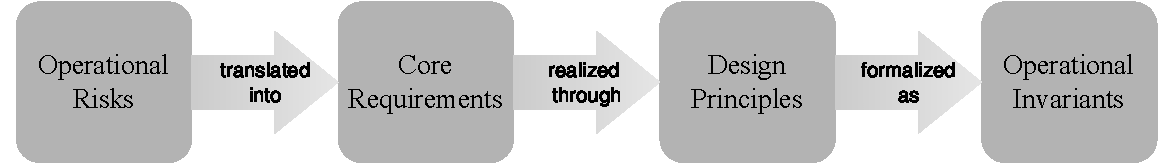
\includegraphics[width=1\linewidth]{figures/Framework.pdf}
    \caption{\hl{Operational Data Foundation Framework.}}
    \label{fig:4-1_framework}
\end{figure}
    


%%%%%%%%%%%%%%%%%%%%%%%%%%%%%%%%%%%%%%%%%%
\subsection{Core Requirements}
\label{sec:core_requirements}

The framework begins by defining the \emph{\hl{core requirements}}. These requirements are not merely desirable properties in a general sense, but the minimum lifecycle-wide guarantees needed for operational viability under constrained SME factory conditions. They provide the basis for the design principles and operational invariants developed in the \mbox{following subsections}.

Six core requirements are defined.


\begin{itemize}
    \item[\textbf{\hl{R1.}}] \textbf{\hl{Continuity}:} %MDPI: Please confirm if the list format and bold should be kept.
    Data continuity should be preserved as far as practicable despite field disruption and connectivity instability. The essential requirement is not momentary acquisition success, but the minimization of gaps and the preservation of recoverable continuity so that the operational record remains usable even when intermediate segments are unstable.

    \item[\textbf{\hl{R2.}}] \textbf{\hl{Governance}:} Source identity, metric semantics, and time semantics should remain stable across collection, normalization, and storage. Data are not operationally usable merely because they exist; they must retain controlled meaning and interpretable context throughout the pipeline.

    \item[\textbf{\hl{R3.}}] \textbf{\hl{Diagnosability}:} Failures should be observable as segment-level discrepancies rather than only as end-to-end symptoms. The requirement is not simply that problems become visible after downstream effects appear, but that the lifecycle location and mode of failure can be identified in a structurally interpretable manner.

    \item[\textbf{\hl{R4.}}] \textbf{\hl{Operability}:} The system should remain maintainable and manageable under constrained staffing and budget conditions. An operational data foundation must therefore be sustainable in day-to-day practice without imposing a structurally excessive maintenance burden or operational complexity.

    \item[\textbf{\hl{R5.}}] \textbf{\hl{Reprocessability}:} Historical data should remain reprocessable for rule changes, KPI revisions, correction, and recovery. Manufacturing data should not be treated as one-time consumables, but as records that can be revisited, recalculated, and reinterpreted as operational needs evolve.

    \item[\textbf{\hl{R6.}}] \textbf{\hl{Evolvability}:} The foundation should accommodate new sources, processes, sites, and applications without breaking the existing structure. Because SME digitalization typically proceeds through incremental onboarding rather than one-time integration, the data foundation must remain structurally open to change and extension.
\end{itemize}

%%%%%%%%%%%%%%%%%%%%%%%%%%%%%%%%%%%%%%%%%%
\subsection{Design Principles}
\label{sec:design_principles}

The core requirements defined above specify what the operational data foundation must guarantee, but not how those guarantees should be realized in design. This subsection therefore presents the key \emph{\hl{design principles}} that translate those requirements into a workable design logic for constrained SME factory conditions. Rather than prescribing specific technologies or implementation choices, these principles define the structural directions needed to sustain the required operational guarantees.

\begin{itemize}
    \item[\textbf{\hl{P1.}}] \textbf{\hl{Continuity responsibility should be placed close to the source:}} If continuity depends primarily on downstream transmission or cloud reachability, it becomes fragile under field disruption and connectivity instability. For this reason, the primary responsibility for preserving continuity should be placed as close to the source as possible through source-near capture, upstream buffering or persistence, and recovery-oriented ingestion logic.

    \item[\textbf{\hl{P2.}}] \textbf{\hl{Raw events should be preserved before abstraction:}} If only transformed outputs are retained, later replay, reinterpretation, and recovery become structurally constrained. Preserving raw events before irreversible abstraction is therefore a fundamental design principle, since rule changes, KPI revision, and correction all depend on access to preserved pre-abstraction records.

    \item[\textbf{\hl{P3.}}] \textbf{\hl{Semantics should be contract-defined:}} If source identity, metric naming, timestamp semantics, unit definition, and transformation logic are left to ad hoc implementation, semantic inconsistency accumulates across the pipeline. The design must therefore define semantics explicitly through controlled contracts, schema discipline, version-aware rules, and clear conventions for identity and time.

    \item[\textbf{\hl{P4.}}] \textbf{\hl{Observability should follow pipeline segments:}} Diagnosability cannot be secured through black-box end-to-end monitoring alone, because operationally meaningful failures must be localizable to specific lifecycle segments. Observability should therefore be structured along the pipeline itself through segment-level checkpoints, stage-level indicators, and explicit discrepancy visibility.

    \item[\textbf{\hl{P5.}}] \textbf{\hl{Responsibilities should be separated by function:}} If acquisition, normalization, storage, and downstream use are tightly coupled, both maintenance burden and change cost rise rapidly. Functional responsibilities should therefore be separated so that components remain structurally independent, interfaces remain replaceable, and modifications in one part do not unnecessarily destabilize the whole.

    \item[\textbf{\hl{P6.}}] \textbf{\hl{Operations should remain lightweight, modular, and open:}} In constrained SME environments, heavy operational structures, costly maintenance models, and vendor dependence undermine long-term viability. The design should therefore remain lightweight in deployment, modular in composition, manageable in maintenance scope, and open to replacement and extension. Where appropriate, open and widely supported components, including open-source tools, can help reduce lock-in and maintenance burden.
    
    \item[\textbf{\hl{P7.}}] \textbf{\hl{Change should be treated as a first-class assumption:}} Changes in KPIs, schemas, rules, source onboarding, and deployment scope are not exceptional events, but normal operating conditions in SME digitalization. The foundation should therefore be designed from the outset to accommodate and organize change through version-aware structures, replay support, incremental onboarding discipline, and \mbox{change-tolerant interfaces}.
\end{itemize}

%%%%%%%%%%%%%%%%%%%%%%%%%%%%%%%%%%%%%%%%%%
\subsection{Operational Invariants}
\label{sec:operational_invariants}

The core requirements and design principles defined above specify what the operational data foundation must guarantee and how those guarantees should be realized. This subsection completes the framework by defining the \emph{\hl{operational invariants}}, that is, the persistent conditions that should hold if the foundation is functioning as intended.

\begin{itemize}
    \item[\textbf{\hl{I1.}}] \textbf{\hl{Durable Capture Invariant:}} An accepted event should obtain durable persistence before any downstream failure can erase it. Continuity should therefore be judged from the point of first durable capture rather than from downstream availability alone.

    \item[\textbf{\hl{I2.}}] \textbf{\hl{Traceability Invariant:}} Every canonical or stored record should remain traceable to its source identity and operational context. Downstream data should not become detached from the source, metadata, and governing semantics that give them meaning.

    \item[\textbf{\hl{I3.}}] \textbf{\hl{Deterministic Normalization Invariant:}} The same raw event under the same contract and version conditions should always produce the same canonical output. Normalization should function as a repeatable and controlled semantic transformation rather than as ad hoc interpretation.

    \item[\textbf{\hl{I4.}}] \textbf{\hl{Segment-Localizable Failure Invariant:}} A failure should become visible as at least one discrepancy within a recognizable lifecycle segment. It should be possible to attribute the problem to a specific segment, such as the source, transmission, preprocessing, loading, storage, or sink, rather than observing it only as a downstream symptom.

    \item[\textbf{\hl{I5.}}] \textbf{\hl{Replayability Invariant:}} Preserved raw data should remain reprocessable for rule changes, KPI revision, correction, and recovery. Historical data should therefore remain usable for later reinterpretation and recomputation, rather than serving only as passive archival material.

    \item[\textbf{\hl{I6.}}] \textbf{\hl{Modular Replacement Invariant:}} Replacing a specific component should not break the semantic chain of the overall foundation. Changes in storage, parsing, transport, or downstream components should not destroy source identity, metric meaning, or replay context across the system.

    \item[\textbf{\hl{I7.}}] \textbf{\hl{Onboarding Consistency Invariant:}} A new source should be incorporable into the existing structure without breaking the prevailing governance discipline. Incremental onboarding should proceed through the same contract, schema, naming, and validation discipline, rather than through an accumulation of ad hoc exceptions.
\end{itemize}

The relationship between the design principles and the invariants is cumulative rather than strictly one-to-one. Some invariants are supported mainly by a single principle, such as P1 for I1 Durable Capture, P2 for I5 Replayability, and P4 for I4 Segment-Localizable Failure. Others require combined design logic: P3 supports I2 Traceability and I3 Deterministic Normalization through contract-defined semantics, P5 supports both I4 and I6 by separating functional responsibilities, and P6 and P7 further support I6 and I7 by enabling modular operation and change-aware onboarding. In this sense, the invariants make the design principles assessable as persistent operational conditions rather than introducing a separate checklist. The broader relationship among SME constraints, risks, requirements, principles, and invariants is synthesized later in Table~\ref{tab:constraint_design_logic}.

These invariants define the persistent conditions by which the framework can be assessed in practice. If requirements declare the guarantees to be achieved and principles define the design logic needed to achieve them, invariants provide the basis for evaluating whether those guarantees remain structurally preserved.

%%%%%%%%%%%%%%%%%%%%%%%%%%%%%%%%%%%%%%%%%%
\subsection{Framework Synthesis}
\label{sec:framework_synthesis}

This subsection synthesizes the framework by reconnecting it to the problem space analyzed in Section~\ref{sec:problem_analysis}. Section~\ref{sec:problem_analysis} showed how constrained SME factory conditions destabilize the general data pipeline lifecycle and generate recurring risks related to continuity, governance, diagnosability, operability, reprocessability, and evolvability. Sections~\ref{sec:core_requirements}--\ref{sec:operational_invariants} then translated those risks into core requirements, design principles, and operational invariants. The purpose of this subsection is to clarify how these layers are systematically linked to the underlying problem structure.

Table~\ref{tab:constraint_design_logic} provides the first synthesis. It shows that constrained SME conditions are not merely a list of deployment difficulties, but recurring operational design problems that can be translated systematically. Each major constraint category gives rise to one or more operational risks; each risk is then expressed as a core requirement, translated into one or more design principles, and made assessable through corresponding invariants. In this way, the table shows how the framework is grounded in recurring structural problems in constrained SME manufacturing.


One particularly important translation highlighted in Table~\ref{tab:constraint_design_logic} is the shift from semantic and interface heterogeneity to governance logic. Here, the central issue is not merely integration, but the need to keep source identity, metric meaning, unit interpretation, and timestamp semantics stable across the pipeline. The framework therefore links this problem to \emph{\hl{R2 Governance}%MDPI: Please confirm if the italics are necessary; if not, please remove them. The following highlights are the same.
}, \emph{\hl{P3 contract-defined semantics}}, and the assessable conditions of \emph{\hl{I2 Traceability}} and \emph{\hl{I3 Deterministic Normalization}}. This translation makes clear that manufacturing data become operationally reliable only when meaning and origin remain stably governed.

A second important translation concerns the shift from change pressure to reprocessability and evolvability logic. Here, the central issue is whether the foundation can remain coherent as KPIs, schemas, sources, and operational rules evolve over time. The framework therefore links this problem to \emph{\hl{R5 Reprocessability}} and \emph{\hl{R6 Evolvability}}, supported by \emph{\hl{P7 change as a first-class assumption}} and assessed through \emph{\hl{I5 Replayability}} and \emph{\hl{I7 Onboarding Consistency}}. This shows that the framework is designed not only for present-time correctness, but also to preserve operational coherence under future change.

Table~\ref{tab:lifecycle_foundation_logic} provides a second synthesis by showing how the framework adds operational meaning to the general data pipeline lifecycle. Under constrained SME conditions, each lifecycle stage must contribute not only to data movement and processing, but also to the guarantees defined by the operational data foundation. The table makes this added meaning explicit by connecting each stage to the relevant risks, requirements, design principles, and invariants. In this way, the general lifecycle is retained as an analytical reference, while its role is sharpened for constrained manufacturing conditions.

\begin{table}[H]
\small
\caption{\hl{From} %MDPI: Please note that changes to the position/size of figures or tables may occur during the production stage. %MDPI: We moved Figures after the first mentioned paragraph in the text, please confirm.
 SME constraints to operational design logic.\label{tab:constraint_design_logic}}
\begin{adjustwidth}{-\extralength}{0cm}
\renewcommand{\arraystretch}{1.2}
\begin{tabularx}{\fulllength}{
>{\raggedright\arraybackslash}X
>{\raggedright\arraybackslash}X
>{\raggedright\arraybackslash}X
>{\raggedright\arraybackslash}X
>{\raggedright\arraybackslash}X}
\toprule
\textbf{SME Constraint} & \textbf{Operational Risk} & \textbf{Requirements} & \textbf{Principles} & \textbf{Invariants} \\
\midrule

Heterogeneous devices and fragmented interfaces
& RSK2 (Governance risk)
& R2 (Governance)
& P3 (Semantics must be contract-defined)
& I2 (Traceability), I3 (Deterministic normalization) \\
\specialrule{0.2pt}{0pt}{0pt}

Add-on sources and partial visibility
& RSK2, RSK6 (Evolvability risk)
& R2, R6 (Evolvability)
& P3, P7 (Change as a first-class assumption)
& I2, I7 (Onboarding consistency) \\
\specialrule{0.2pt}{0pt}{0pt}

Unstable connectivity and constrained sensing
& RSK1 (Continuity risk)
& R1 (Continuity)
& P1 (Continuity responsibility must be placed close to the source)
& I1 (Durable capture) \\
\specialrule{0.2pt}{0pt}{0pt}

Weak cross-segment observability
& RSK3 (Diagnosability risk)
& R3 (Diagnosability)
& P4 (Observability must follow pipeline segments)
& I4 (Segment-localizable failure) \\
\specialrule{0.2pt}{0pt}{0pt}

Limited staff and high maintenance burden
& RSK4 (Operability risk)
& R4 (Operability)
& P6 (Operations must remain lightweight, modular, and open)
& I6 (Modular replacement) \\
\specialrule{0.2pt}{0pt}{0pt}

Weak raw-data preservation
& RSK5 (Reprocessability risk)
& R5 (Reprocessability)
& P2 (Raw events must be preserved before abstraction)
& I5 (Replayability) \\
\specialrule{0.2pt}{0pt}{0pt}

Tight functional coupling across the pipeline
& RSK3, RSK4, RSK6
& R3, R4, R6
& P5 (Responsibilities must be separated by function)
& I4, I6 \\
\specialrule{0.2pt}{0pt}{0pt}

Frequent KPI, rule, schema, and source changes
& RSK5, RSK6
& R5, R6
& P7
& I5, I7 \\
\specialrule{0.2pt}{0pt}{0pt}

Budget sensitivity and lock-in concerns
& RSK4, RSK6
& R4, R6
& P6
& I6, I7 \\
\bottomrule
\end{tabularx}
\end{adjustwidth}
\end{table}




\vspace{-8pt}





\begin{table}[H]
\caption{\hl{Mapping} %MDPI: Please confirm if the alignment should be kept.
 the general data pipeline lifecycle to the operational foundation logic.\label{tab:lifecycle_foundation_logic}}
\begin{adjustwidth}{-\extralength}{0cm}
\renewcommand{\arraystretch}{1.4}
\begin{tabularx}{\fulllength}{
>{\raggedright\arraybackslash}p{0.16\fulllength}
>{\raggedright\arraybackslash}p{0.24\fulllength}
>{\raggedright\arraybackslash}X
>{\raggedright\arraybackslash}p{0.12\fulllength}
>{\raggedright\arraybackslash}p{0.10\fulllength}
>{\raggedright\arraybackslash}p{0.10\fulllength}}
\toprule
\textbf{General Lifecycle Stage} & \textbf{Added Operational Meaning} & \textbf{Related Risks} & \textbf{Requirements} & \textbf{Principles} & \textbf{Invariants} \\
\midrule

Data sources
& Stable source identity
& RSK2, RSK6
& R2, R6
& P3, P7
& I2, I7 \\

Data ingestion
& Source-near continuity and intake control
& RSK1, RSK2
& R1, R2
& P1, P3
& I1, I2 \\

Data transmission
& Recoverable transfer and visible discrepancies
& RSK1, RSK3
& R1, R3
& P1, P4
& I1, I4 \\

Data preprocessing
& Contract-defined and deterministic transformation
& RSK2, RSK6
& R2, R6
& P3, P7
& I2, I3, I7 \\

Data loading
& Controlled persistence with replay context
& RSK5, RSK6
& R5, R6
& P2, P7
& I5, I7 \\

Data storage
& Replay-ready and replaceable persistence
& RSK4, RSK5
& R4, R5
& P2, P6
& I5, I6 \\

Data sinks
& Governed downstream reuse
& RSK2, RSK5
& R2, R5
& P3, P7
& I2, I5 \\

Monitoring and management
& Lifecycle-wide observability and maintainability
& RSK3, RSK4
& R3, R4
& P4, P6
& I4, I6 \\

\bottomrule
\end{tabularx}
\end{adjustwidth}
\end{table}



One especially revealing example is the reinterpretation of the transmission stage. In generic pipeline discussions, transmission is often treated as a routine internal link between ingestion and subsequent processing. In constrained SME factory conditions, however, the path from field devices to gateways, edge systems, servers, and cloud systems is often exposed to intermittent connectivity, limited bandwidth, battery constraints, delayed recovery, and relay dependence. Transmission therefore becomes a distinct operational segment in which continuity and diagnosability are directly tested. For this reason, Table~\ref{tab:lifecycle_foundation_logic} assigns the transmission stage the added meanings of recoverable transfer and segment-aware discrepancy visibility, linking it to \emph{\hl{R1 Continuity}}, \emph{\hl{R3 Diagnosability}}, \emph{\hl{P1 source-near continuity}}, \emph{\hl{P4 segment-based observability}}, \emph{\hl{I1 Durable Capture}}, and \emph{\hl{I4 \mbox{Segment-Localizable Failure}}}.

Taken together, Table~\ref{tab:constraint_design_logic} translates constrained SME conditions into operational design logic, while Table~\ref{tab:lifecycle_foundation_logic} shows how that logic refines the interpretation of the general data pipeline lifecycle under real manufacturing constraints. The result is a single analytical structure that connects the problem space, framework logic, and lifecycle interpretation. This synthesis also provides the basis for reading the field implementation in Section~\ref{sec:field_implementation} and the evidence-based assessment in Section~\ref{sec:framework_evaluation}.

The same synthesis also suggests how the framework can be interpreted in multi-plant or distributed edge--cloud settings. In such settings, scalability is not only a matter of adding more devices, pipelines, or records; it depends on whether the same operational invariants remain valid across sites. Source identities and metric semantics must remain governed across factories, local edge-side capture must preserve continuity despite site-level instability, failures must remain localizable to lifecycle segments, and preserved raw records must remain reprocessable under revised rules or KPIs. Thus, the scalability of an operational data foundation depends on preserving its operational guarantees across distributed sites, rather than merely expanding the technical infrastructure.

%%%%%%%%%%%%%%%%%%%%%%%%%%%%%%%%%%%%%%%%%%
%%%%%%%%%%%%%%%%%%%%%%%%%%%%%%%%%%%%%%%%%%
\section{Field Implementation}
\label{sec:field_implementation}

This section describes how the proposed framework was instantiated in a real SME manufacturing setting. It first introduces the deployment setting, then explains the field-side acquisition and edge architecture, the cloud-side processing path, and the resulting operational use.

%%%%%%%%%%%%%%%%%%%%%%%%%%%%%%%%%%%%%%%%%%
\subsection{Deployment Setting}
\label{sec:deployment_setting}




The empirical setting of this study was the Idang Food yakgwa plant, one of several OEM factories managed by ONGOING, an F\&B company operating across multiple production sites. The deployment was therefore designed not as an isolated factory pilot, but as the first field implementation of a broader architecture in which operational data from multiple factories could be collected locally and managed through a shared cloud-side structure. In this sense, Idang Food was selected not only as a practical implementation site, but also as a representative case through which this study examines how an operational data foundation can be established under constrained SME manufacturing conditions.

The plant's production flow included raw-material receiving, weighing, mixing, forming, frying, coating, cooling, inner packaging, detection, outer packaging, and storage. Yet the main challenge at the site did not lie simply in the number of stages. Operationally relevant states were distributed across different rooms, devices, and tasks, while production and quality management depended heavily on manual records and worker judgment. Process conditions were not accumulated as connected records, weighing-related checks remained strongly operator-dependent, and environmental histories across process and storage zones were difficult to preserve and compare over time. As a result, when abnormal conditions or quality issues emerged, the plant did not lack observations in an absolute sense; rather, it lacked continuous and reusable operational records that could support traceability and later interpretation.

This made the site suitable for the present study. Idang Food reflected several conditions that commonly characterize constrained SME factories: heterogeneous and partly non-networked sources, fragmented process visibility, limited internal connectivity, and restricted operational slack for day-to-day technical management. Under such conditions, an operational data foundation could not be assumed to arise simply from downstream software or cloud connectivity. It first had to be built from the field upward by making process states recordable, collectable, and sustainable as data under actual \mbox{production constraints}.

The field deployment took the form of an actual on-site installation and system realization rather than a conceptual design exercise. The study did not begin with an already prepared digital source environment; instead, it proceeded by physically establishing one inside the factory through sensor placement, gateway configuration, and edge-side deployment. Figure~\ref{fig:5-1_factory} presents this implementation context by showing the production environment together with representative sensing and edge elements installed in the field. This point is important because the case demonstrates not only that an operational data foundation was conceptually proposed, but also that its source-side basis was concretely built and operated in a constrained SME factory. Through that installation, the plant acquired the initial operational foothold required for continuity, traceability, and subsequent cloud-side integration.
\vspace{-3pt}
\begin{figure}[H]
   % \centering
    
\includegraphics[width=1\linewidth]{figures/Factory.pdf}
    \caption{\hl{Factory} %MDPI: We moved Figures after the first mentioned paragraph in the text, please confirm.
 layout with representative sensing and edge deployment.}%MDPI: Please confirm whether an explanation of the different colors and red box needs to be added to the figure caption.
    \label{fig:5-1_factory}
\end{figure}
Accordingly, the role of Idang Food in this study was twofold. At the factory level, it provided a realistic constrained environment in which fragmented sources, manual practices, and brownfield conditions had to be handled in practice. At the system level, it served as the first implementation site of an architecture intended to support factory-to-cloud data flow and centralized multi-factory management. For this reason, the next subsection begins with field data acquisition and the edge architecture, because the first requirement of the operational data foundation was to explain how field data were physically captured and operationally secured at the factory before being forwarded into the broader \mbox{cloud-side system}.


%%%%%%%%%%%%%%%%%%%%%%%%%%%%%%%%%%%%%%%%%%
\subsection{Field Data Acquisition and Edge Architecture}
\label{sec:field_acquisition_edge}


The factory-side acquisition layer was implemented as an edge-centered intake stack that received field data within the plant, preserved them locally, and then forwarded them to the cloud event pipeline. Because the plant did not provide a uniform network-native source environment, and because stable plant-wide connectivity could not be assumed across distributed process areas, the architecture was organized around a local edge boundary rather than direct source-to-cloud transmission.

LoRaWAN, a low-power wide-area communication approach well suited to distributed sensing, was selected as the field communication network for this deployment. This choice reflected the actual plant environment: the production areas did not provide wired LAN coverage, and stable Wi-Fi-based collection could not be assumed across the factory. Alternatives such as Wi-Fi HaLow and Zigbee were considered less practical for this deployment context: Wi-Fi HaLow can also support long-range IoT connectivity, but would have required additional compatible access-point infrastructure, while Zigbee would have increased reliance on mesh coverage and repeater placement across rooms and storage areas. In relation to R1 Continuity, LoRaWAN was selected as a practical option for recoverable field event collection under constrained communication paths, because it reduced dependence on plant-wide local network availability and dense in-factory communication infrastructure. LoRaWAN therefore provided a feasible means of collecting distributed field events without extensive wiring while keeping the gateway--edge path locally controlled within the factory.

As shown in Figure~\ref{fig:edge}, the implemented architecture was organized into three zones: the in-factory field layer on the left, the internal edge stack at the center, and the cloud broker boundary on the right. Field events were transmitted over LoRa to the gateway, handled by ChirpStack Gateway Bridge and ChirpStack Server, relayed through an MQTT broker, and then accepted by edge-side services. On the edge node, the MQTT logger and source-specific collectors wrote accepted records into local SQLite stores before any cloud delivery was assumed. This made the acquisition path explicit---field transmission, gateway reception, LoRaWAN handling, MQTT relay, edge logging, and upper-layer forwarding were treated as separate steps---and established the edge node as the first stable intake and persistence boundary of the system.

\begin{figure}[H]
    %\centering
    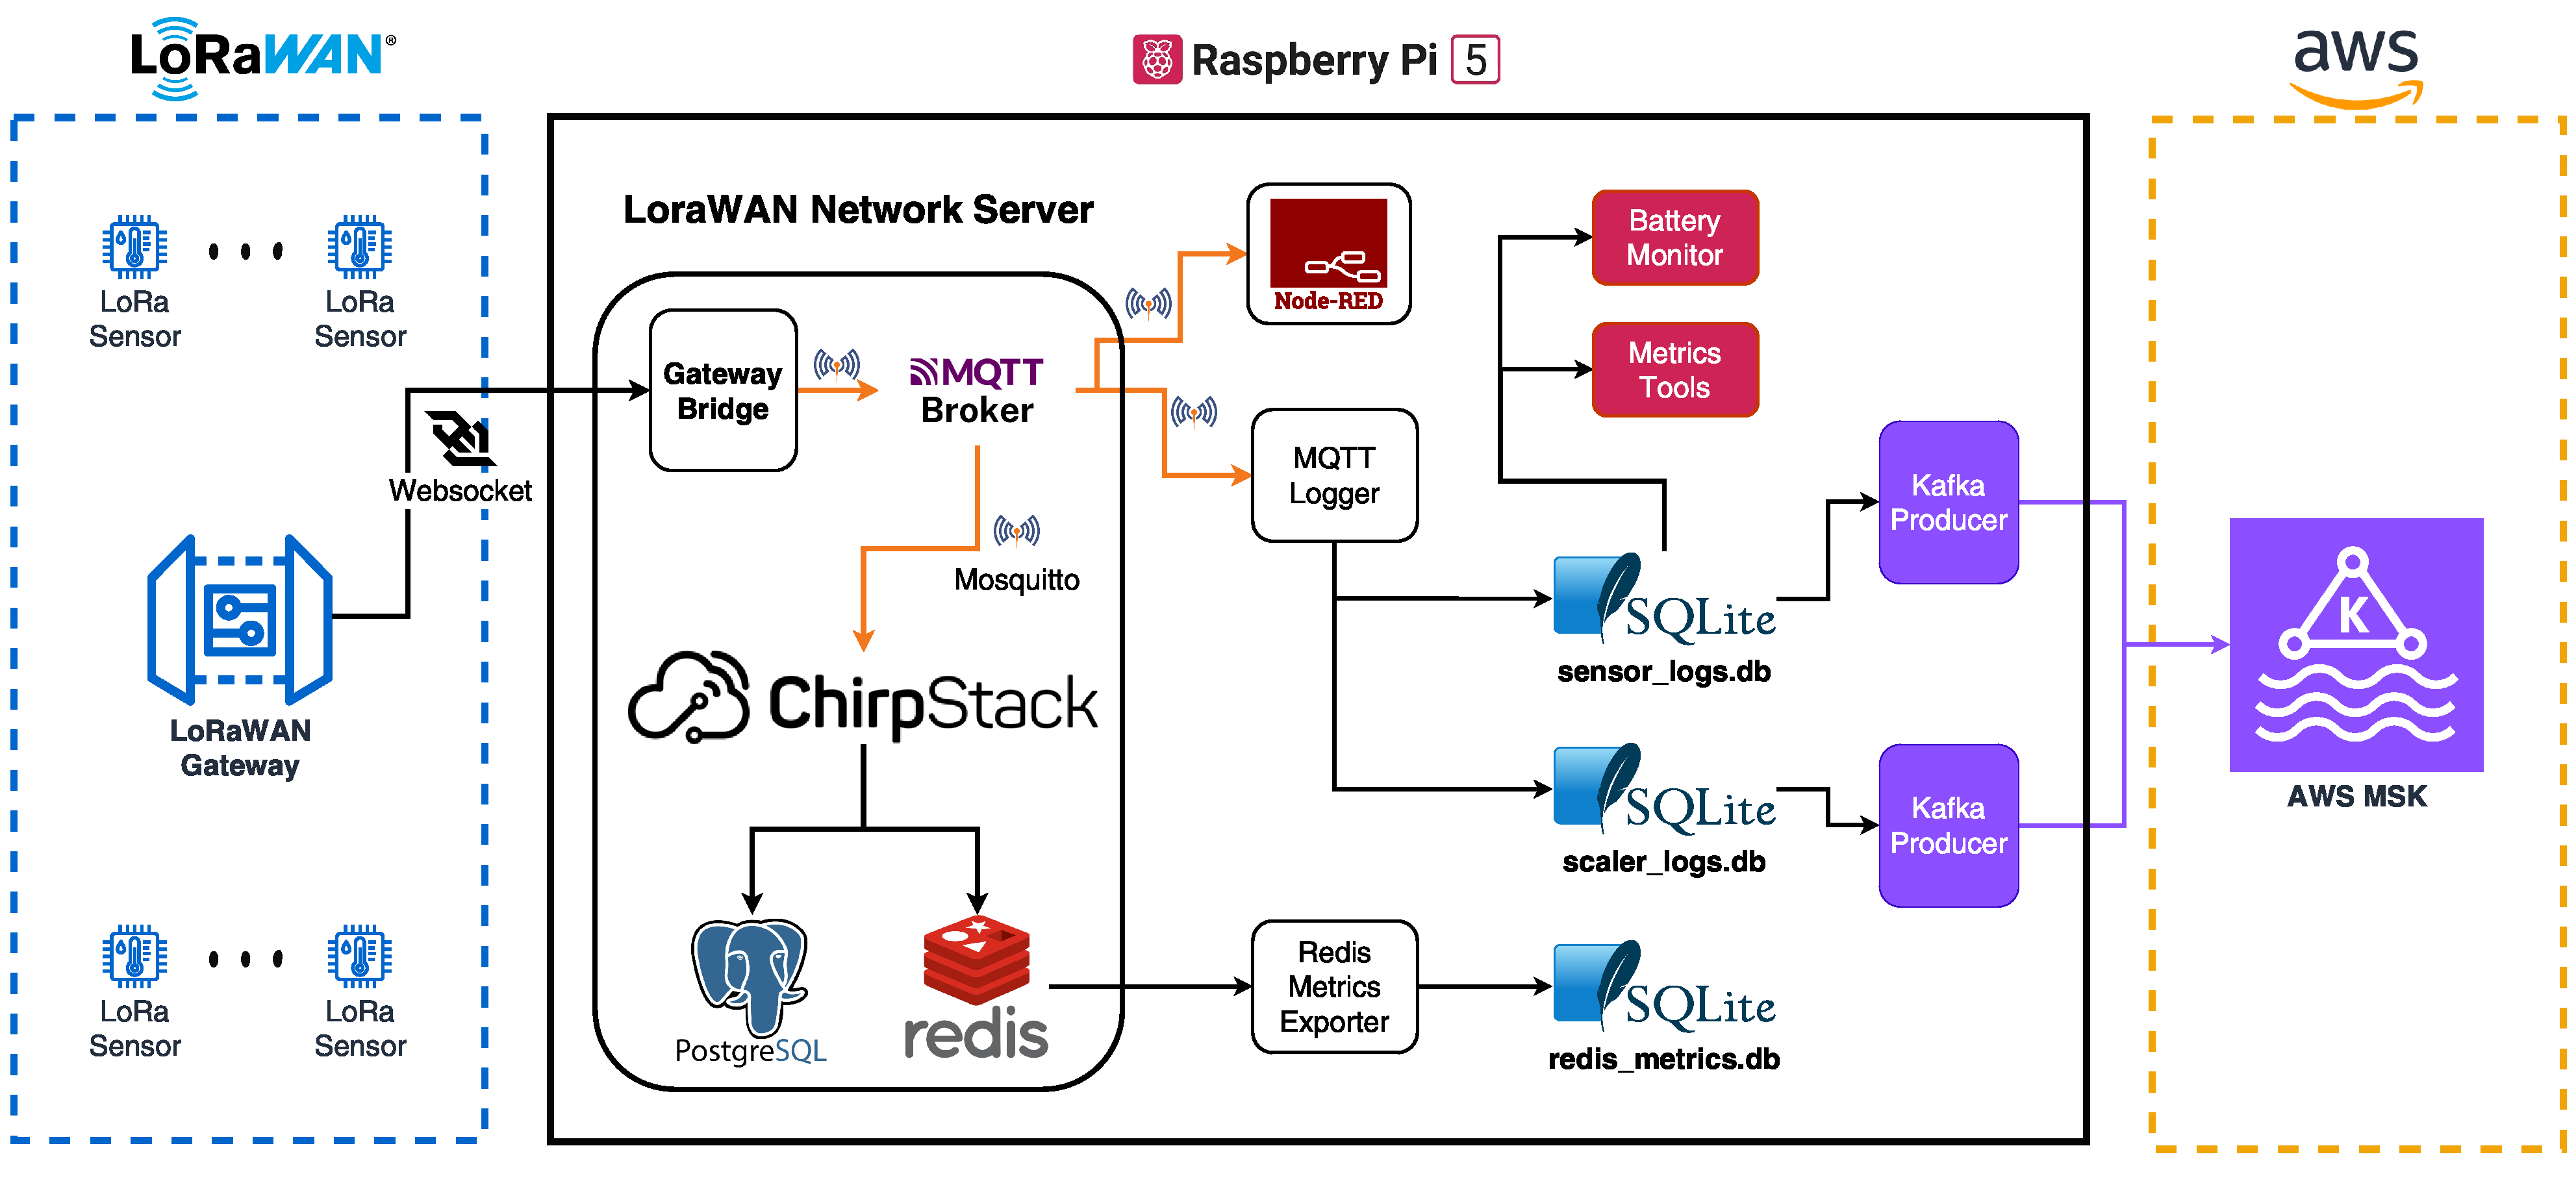
\includegraphics[width=1\linewidth]{figures/Edge_Architecture.pdf}
    \caption{\hl{Edge} %MDPI: Please confirm whether an explanation of the arrows and different colors needs to be added to the figure caption.
 architecture for field data acquisition.}
    \label{fig:edge}
\end{figure}

The edge stack also accommodated heterogeneous source conditions, rather than only native wireless sensor uplinks. A representative example was the production electronic scale, which did not provide native network communication and exposed only a printer port as its available output interface. To incorporate the device without replacement, that port was connected to the Raspberry Pi through an RS232 serial link. A dedicated daemon collector parsed the incoming weighing values, stored them locally, and then transmitted them through a LoRa device attached to the Raspberry Pi so that they could enter the same acquisition path as other field events. In practical terms, this flow can be summarized as \emph{Scale $\rightarrow$ RS232 $\rightarrow$ RPi $\rightarrow$ LoRa}. This shows that the edge architecture could absorb non-networked legacy equipment as well as standard wireless sensor uplinks within the same factory-side event flow.

Once accepted and retained at the edge, the records were forwarded by producer services to the cloud broker layer. In the broader architecture, this upstream path was organized around Kafka-based streaming, including AWS MSK on the cloud side, so that raw events from each factory could be published into a shared event pipeline for subsequent parsing, normalization, and persistence. The next subsection explains this cloud-side processing path.






%%%%%%%%%%%%%%%%%%%%%%%%%%%%%%%%%%%%%%%%%%
\subsection{Cloud Processing and Event Flow}
\label{sec:cloud_processing}


On top of the field acquisition layer, the system implemented a cloud-side processing path that received raw events from factory edges, routed them through a brokered stream architecture, and transformed them into persistent and service-ready records. Multiple factory-originated event streams were forwarded to the AWS cloud and published into Kafka topics in the MSK cluster, where subsequent stages handled normalization, derivation, persistence, and operational consumption. Figure~\ref{fig:cloud_architecture} presents this deployment-level structure by showing how data from multiple factories converged within a shared AWS-based cloud environment and entered a common brokered processing path. In this way, the cloud layer served not as a single application endpoint, but as a staged processing structure connecting multi-factory intake to downstream use.

\begin{figure}[H]
    %\centering
    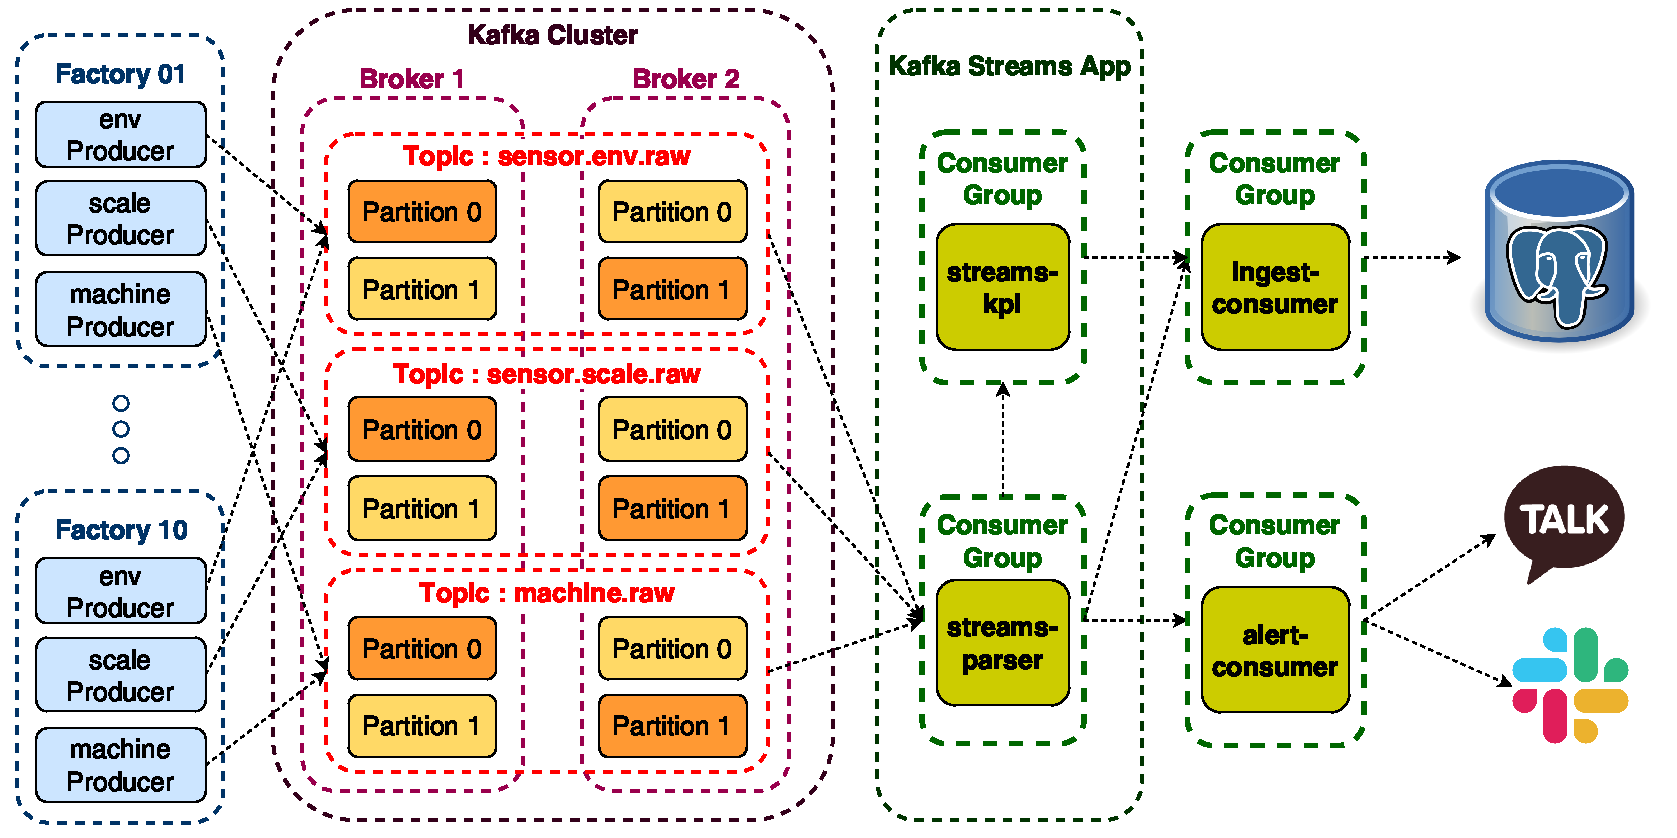
\includegraphics[width=1\linewidth]{figures/Cloud_Architecture.pdf}
    \caption{\hl{Cloud-side} %MDPI: Please confirm whether an explanation of the arrows and different colors needs to be added to the figure caption.
 processing architecture.}
    \label{fig:cloud_architecture}
\end{figure}

Within this cloud path, raw factory events first entered broker topics such as \texttt{\hl{sensor.env.raw}}, \texttt{\hl{sensor.scale.raw}}, and \texttt{\hl{machine.raw}}. %MDPI: Please confirm the font format should be kept.
These raw topics were consumed by the parser stream, which decoded heterogeneous payloads, mapped sources, unified metrics, normalized timestamps, applied deduplication, and produced canonical events for downstream use. On top of this normalized stream, KPI processing and alert-side consumption proceeded as separate downstream paths: KPI streams generated derived indicators such as production quantity and yield, while alert consumers used the same governed event basis to detect conditions requiring notification or intervention. Finally, ingest consumers persisted the normalized and derived outputs to the database layer for later dashboard and analytical use. In this way, the cloud path functioned as a staged transformation flow through which heterogeneous raw messages were converted into governed and reusable operational records.

A central design objective of this layer was functional decoupling. Factory-side producers were able to publish raw events to the broker without depending directly on parser execution, KPI computation, alert handling, or database ingestion. This separation reduced failure propagation across stages and made the system easier to modify as rules, sources, and downstream requirements evolved. In practical terms, the broker layer provided a shared event boundary through which intake, interpretation, derivation, persistence, and service consumption could remain structurally separated.




The parser stream concentrated the semantic normalization responsibility of the cloud path. Rather than allowing later components to interpret device-specific payload structures independently, the system converted heterogeneous source messages into a governed common form at this stage. In this implementation, \hl{\texttt{source\_id}} functioned as the canonical identifier of each operational source by organizing identity around controlled attributes such as tenant, line, process, device type, and metric, while timestamp semantics were stabilized by distinguishing \texttt{\hl{event\_time}}, \texttt{\hl{edge\_ingest\_time}}, and \texttt{\hl{db\_ingest\_time}} as separate time axes with different operational roles. This prevented ambiguity in ordering and interpretation and kept downstream processing aligned with a consistent \mbox{semantic discipline}.
 
 


After canonicalization, KPI computation was intentionally performed in the stream layer rather than deferred to dashboard query time. If production quantity, yield, and related indicators had been computed repeatedly from raw or lightly processed records at query time, each view request would have required additional aggregation and business-rule evaluation over a larger event set. By computing these indicators continuously from the normalized stream and persisting the resulting outputs as ready-to-use records, the system shifted repeated query-time work into incremental event-time processing. This reduced dashboard-side computational burden, simplified query logic, and supported more stable low-latency operational views. At the same time, alert consumers could react to the same governed event basis without overloading either the parser or the \mbox{persistence layer}.

Persistent storage was handled through ingest consumers. These consumers received already normalized or derived events and wrote them into the database without reintroducing business logic at the persistence boundary. As a result, semantic interpretation remained in the parser layer, derived computation remained in the KPI stream, alert-side reaction remained in dedicated consumers, and the storage path remained focused on durable append-oriented persistence. This separation of responsibilities made the cloud-side stack easier to reason about and more robust to later changes in processing rules or downstream interfaces.

Taken together, the cloud-side processing path completed the second half of the operational data foundation. If the field edge established source-near acceptance and local durability, the cloud layer provided brokered multi-factory intake, governed normalization, separated derivation and alert handling, and service-ready persistence. The result was a processing architecture that did not expose raw heterogeneous payloads directly to downstream services, but instead converted them into controlled operational records that could support dashboards, alerts, traceability, and future analytical extension.



%%%%%%%%%%%%%%%%%%%%%%%%%%%%%%%%%%%%%%%%%%
\subsection{Operational Use}
\label{sec:operational_use}

The implementation extended beyond data capture and cloud-side processing into an operational layer through which plant personnel could observe conditions and respond when necessary. This layer mattered because the system was not intended to remain merely a background pipeline. Instead, it was designed to make governed operational records directly usable in day-to-day manufacturing practice and thereby connect the data foundation to actual plant awareness and intervention.

Dashboards translated processed records into operational views suitable for both operators and managers. Rather than exposing raw signals alone, the system presented current conditions, recent trends, source health, packet reception quality, and derived indicators in forms that supported routine monitoring. This changed the practical mode of work at the plant. Before digitalization, condition checking depended heavily on manual records, fragmented local observation, and worker judgment. With the implemented layer, plant personnel could instead rely on a shared and continuously updated reference for process and environmental conditions, reducing exclusive dependence on tacit judgment and making operational awareness more consistent and reviewable.

Alerting formed the intervention path of this layer. When operationally meaningful conditions were detected, for example, fryer oil temperature departing from its expected range, storage-area temperature rising sharply during extreme summer heat, prolonged silence from a source, or battery-related degradation affecting sensor reliability, the system generated asynchronous alerts so that personnel could respond in time. In this design, alerts were not merely an accessory to dashboards, but the mechanism through which monitored states became actionable events. The resulting loop can be understood as observe--detect--notify--act.

The implemented layer also reached the point of machine-side intervention capability. The system was built to support actual device power control in the field, showing that the operational data foundation did not remain limited to passive observation and notification. Although this study does not center on closed-loop control automation itself, this capability is important because it shows that the same governed data basis could already support downstream action as well as monitoring. Taken together, the operational layer demonstrates that the implemented system functioned not merely as a data pipeline, but as a practical interface connecting visibility, alerting, human response, and intervention on a common operational data foundation.



%%%%%%%%%%%%%%%%%%%%%%%%%%%%%%%%%%%%%%%%%%
%%%%%%%%%%%%%%%%%%%%%%%%%%%%%%%%%%%%%%%%%%
\section{Evaluation of the Framework}
\label{sec:framework_evaluation}

This section evaluates whether the proposed framework functioned as an operational data foundation in a real manufacturing setting. Rather than emphasizing benchmark performance or algorithmic accuracy, the evaluation examines how the six framework requirements became visible in the implemented system and its operational history. Accordingly, Section~\ref{sec:framework_compliance} reviews requirement-wise evidence, and Section~\ref{sec:lora_reliability} presents a representative field case that illustrates more concretely how the framework became visible in \mbox{actual operation}.


%%%%%%%%%%%%%%%%%%%%%%%%%%%%%%%%%%%%%%%%%%
\subsection{Framework Compliance}
\label{sec:framework_compliance}

This subsection examines framework compliance across the six core requirements defined in Section~\ref{sec:odff}. Rather than reducing each requirement to a single metric, it considers multiple forms of representative evidence, summarizes them in Table~\ref{tab:requirement_compliance_snapshot}, and interprets their operational meaning.


\begin{table}[H]
\caption{Requirement-wise compliance snapshot.\label{tab:requirement_compliance_snapshot}}
\renewcommand{\arraystretch}{1.15}
\begin{tabularx}{\textwidth}{
>{\raggedright\arraybackslash}p{0.30\textwidth}
>{\raggedright\arraybackslash}X}
\toprule
\textbf{Requirement} & \textbf{Representative Evidence} \\
\midrule

Continuity
& local persistence, recovery path, gap reduction \\

Governance
& source identity, canonical semantics, time separation \\

Diagnosability
& segment-wise visibility, stage discrepancy checks \\

Operability
& modular stack, monitoring and intervention points \\

Reprocessability
& raw-like retention, layered persistence \\

Evolvability
& common event contract, extensible onboarding \\

\bottomrule
\end{tabularx}
\renewcommand{\arraystretch}{1.0}
\end{table}



\textbf{\hl{Continuity}%MDPI: Please confirm if the bold formatting is necessary; if not, please remove it. The following highlights are the same.
} was assessed not as perfect packet arrival, but as the preservation of a recoverable operational record under unstable field conditions. In the implemented system, gateway reception, edge-side logging, downstream ingest, and database persistence were observable as separate stages, allowing continuity to be examined through persisted-to-expected ratios and before--after recovery patterns. As summarized in Table~\ref{tab:continuity_improvement_summary}, the field intervention substantially improved the persisted-to-expected ratio. This compact summary provides the requirement-level evidence for R1 Continuity, while the detailed diagnosis and intervention process is discussed as a representative field case in Section~\ref{sec:lora_reliability}.

\begin{table}[H]
\caption{Summary of continuity improvement after field intervention.}
\label{tab:continuity_improvement_summary}
\centering
\begin{tabularx}{\textwidth}{
>{\raggedright\arraybackslash}p{0.25\textwidth}
>{\centering\arraybackslash}X
>{\centering\arraybackslash}X
>{\centering\arraybackslash}X}
\toprule
\textbf{Period} & \textbf{Received Events} & \textbf{Expected Events} & \textbf{Reception Ratio} \\
\midrule
Before intervention & 15,870 & 48,000 & 33.1\% \\
After intervention & 45,600 & 48,000 & 95.0\% \\
\bottomrule
\end{tabularx}
\end{table}


\textbf{\hl{Governance}} was evaluated in terms of whether heterogeneous field events were brought under a stable semantic discipline across collection, normalization, and storage. In the implemented system, source identity was governed through \texttt{source\_id}, while the parser stage fixed metric definitions, timestamp interpretation, and normalization rules before downstream use. The distinction among \texttt{event\_time}, \texttt{edge\_ingest\_time}, and \texttt{db\_ingest\_time} prevented ambiguity between occurrence time, pipeline reference time, and persistence time. In addition, the separation of raw-like event storage, source metadata, and derived KPI layers preserved a clear boundary between operational records and business-level abstraction. Taken together, these structures show that governance was achieved through controlled meaning, traceable identity, and stable interpretation across the pipeline.

\textbf{\hl{Diagnosability}} was assessed in terms of whether degradation remained a black-box symptom or became visible as a discrepancy localizable to specific lifecycle segments. Because gateway-visible counts, local edge logs, parser and consumer stages, and database persistence counts could be compared, the same symptom of ``too little data'' could be interpreted as different failure modes depending on where the discrepancy first appeared. In some periods, gateway-visible counts were already far below expectation, directing attention to upstream collection and communication. In other cases, the divergence widened only after gateway reception, indicating the need to inspect downstream processing or storage. This segment-wise visibility was especially important in the LoRa case discussed in Section~\ref{sec:lora_reliability}, where the main source of degradation could be narrowed to the communication and configuration layer rather than misread as a parser or database issue.

\textbf{\hl{Operability}} was reflected not simply in whether the system could be made to run, but in whether it could be deployed, inspected, adjusted, and maintained under limited staffing and maintenance capacity. The implemented structure separated field-side acquisition, gateway and network services, edge persistence, cloud-side stream processing, database storage, and dashboard and alert interfaces by function, thereby reducing unnecessary coupling among acquisition, normalization, persistence, derivation, and presentation. In practice, interventions such as rejoin handling, communication-parameter adjustment, logging verification, interval tuning, packet comparison, dashboard inspection, and alert-based response could be carried out at the relevant layer without redesigning the system as a whole. This indicates that the foundation remained operationally manageable as a field system rather than merely as a one-time prototype.

\textbf{\hl{Reprocessability}} was assessed in terms of whether collected records remained available for later reinterpretation, recalculation, correction, and recovery, rather than being consumed only by the current dashboard or rule logic. The implemented system avoided transformed-only persistence by separating raw-like event storage, source metadata, and derived KPI layers, so that later parser revision or KPI redefinition did not depend on reconstructing already abstracted outputs. During operation, replay was executed after revising the yield calculation rule, and the yield KPI was recomputed from preserved raw-like production and weighing records. Because the original payload fields, source identifiers, event-time values, and derived-layer separation remained intact, the revised yield KPI was produced without recollecting field data. Historical data therefore remained available for rule revision, retrospective audit, recomputation, and reconstruction of prior operational states. More importantly, the retained records were preserved in a structure that supported replay-oriented reinterpretation, which is the practical core of reprocessability in a changing manufacturing environment.

\textbf{\hl{Evolvability}} was evaluated in terms of whether the structure could absorb new source types, process-specific measurements, monitoring functions, KPI logic, and downstream services without breaking its governance discipline. This property was reflected not only in the architecture itself, but also in the system's actual expansion history. The implemented foundation accommodated heterogeneous environmental sensors, a retrofitted legacy scale, cloud-side stream processing, derived KPI generation, and dashboard and alert functions within a common event flow governed by shared identity and normalization rules. Because the structure was organized around an explicit event contract, parser-stage normalization, layered persistence, and modular separation of responsibilities, extensions could be handled mainly through onboarding rules, parser updates, and additional downstream consumers rather than through full pipeline redesign. This indicates that the framework supported staged expansion while preserving semantic and operational coherence.

Taken together, the evidence above indicates that the proposed framework was realized not only as a conceptual structure, but also as an operational one in the field. To make this more concrete, the next subsection examines a representative field case through which the framework's practical relevance can be seen in actual operation.



%%%%%%%%%%%%%%%%%%%%%%%%%%%%%%%%%%%%%%%%%%
\subsection{Operational Case: LoRa Reliability Improvement}
\label{sec:lora_reliability}



A field data foundation does not remain operationally reliable simply because it has once been installed. In practice, reception quality, device condition, battery state, wireless configuration, and usage patterns continue to change over time. For this reason, the value of the proposed framework lies not in whether it delivered perfect behavior from the outset, but in whether emerging failures could be detected, localized, and corrected in an operationally meaningful way. This subsection presents a representative field case in which severe degradation in periodic uplink reception was diagnosed and improved within the implemented foundation.

During the early operational period, plant-wide periodic collection failed to sustain its expected level. Reception across multiple monitored sensor sets dropped to roughly 33\%, daily persisted events were 15{,}870 out of an expected 48{,}000, and repeated no-data intervals of 2--5 h appeared across several monitored periods. This was not merely a matter of reduced communication quality. It directly weakened line-level visibility, reduced confidence in dashboard and alert outputs, and undermined the continuity of the operational record on which later interpretation depended.

Because the implemented system did not rely solely on final database status, the degradation could be interpreted as a segment-wise discrepancy rather than as a vague end-to-end symptom. Expected transmissions, gateway-visible events, edge or local logs, ingest-stage counts, and database persistence counts could be examined together. Figure~\ref{fig:failure_localization} summarizes this diagnostic logic as a sequence of adjacent-stage discrepancy checks, in which the first substantial gap indicates the most likely failure boundary. As shown by the actual segment-wise counts in Table~\ref{tab:segmentwise_event_counts}, the main loss had already occurred before parsing and database persistence: in a representative 24 h window, only about 16{,}400 events were visible at the gateway, whereas downstream retention from gateway-visible events to database persistence remained consistently high at roughly 98--99\%. This observed pattern indicated that the dominant loss was occurring before the parser and database layer, making the collection and communication segment the primary locus of investigation.


\begin{figure}[H]
    %\centering
    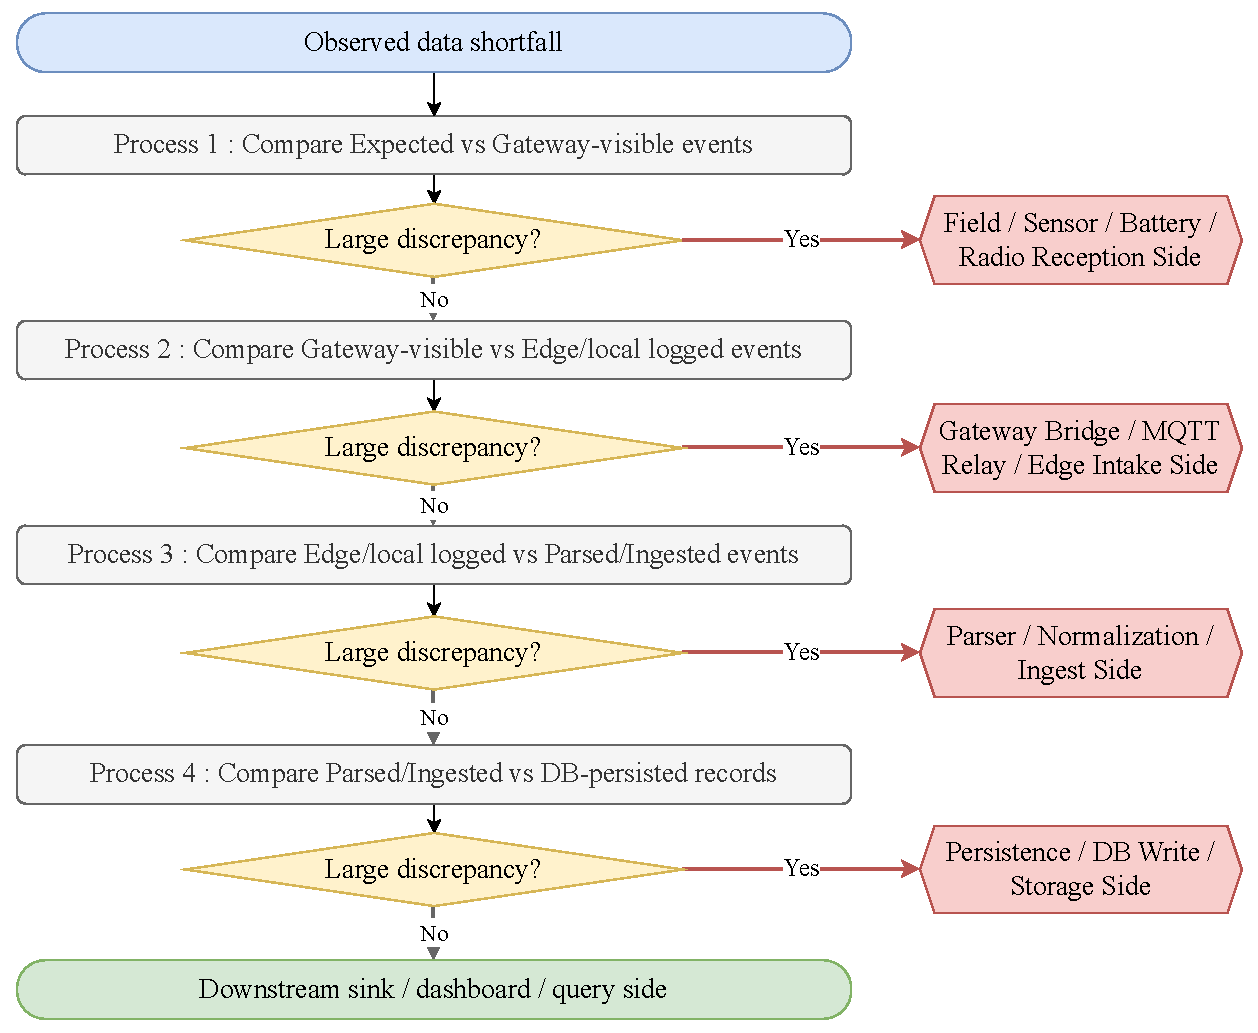
\includegraphics[width=0.99\linewidth]{figures/failure_localization.pdf}
    \caption{\hl{Segment-wise} %MDPI: Please confirm whether an explanation of the arrows and different colors needs to be added to the figure caption.
 failure localization through adjacent-stage discrepancy checks.}
    \label{fig:failure_localization}
\end{figure}

\vspace{-8pt}

\begin{table}[H]
\caption{Event counts across pipeline segments during reception degradation.\label{tab:segmentwise_event_counts}}
\renewcommand{\arraystretch}{1.1}
\begin{tabularx}{\textwidth}{
>{\raggedright\arraybackslash}p{0.37\textwidth}
>{\raggedleft\arraybackslash}X
>{\raggedleft\arraybackslash}X
>{\raggedleft\arraybackslash}X}
\toprule
\textbf{Stage/Metric} & \textbf{Expected} & \textbf{Observed} & \textbf{Ratio (\%)} \\
\midrule

Expected transmissions
& 48{,}000
& --
& -- \\

Gateway-visible events
& 48{,}000
& 16{,}400
& 34.2 \\

Edge/local logged events
& 16{,}400
& 16{,}120
& 98.3 \\

Parsed/Ingested events
& 16{,}120
& 15{,}980
& 99.1 \\

DB-persisted events
& 15{,}980
& 15{,}870
& 99.3 \\

\bottomrule
\end{tabularx}
\renewcommand{\arraystretch}{1.0}
\end{table}


The subsequent diagnosis localized the main bottleneck not to parser failure or database loss, but to the LoRa communication and configuration layer. The problem was not simply a general reduction in signal strength, but a network condition in which frequent periodic confirmed uplinks depended on downlink acknowledgements under limited active-channel availability. When acknowledgements were delayed or missed, retransmissions accumulated, channel contention increased, and reception became uneven across devices. In addition, stale device participation state in part of the fleet required rejoin recovery before stable collection could resume. The diagnosed issue was therefore a concrete reception bottleneck in the LoRa network path itself: ACK-dependent uplink behavior, limited effective channel use, and device-state instability were jointly degrading collection before downstream processing began.

Once the likely bottleneck had been localized, the response proceeded through targeted intervention rather than unguided trial and error. The main adjustments included reducing confirmed-mode dependence, expanding active channels, performing device rejoin, tuning transmission-related parameters, and refining monitoring intervals. After these adjustments, collection stability improved markedly. Packet reception increased from approximately 33\% to 95\%, daily persisted events rose from 15{,}870 to 45{,}600, extended no-data intervals decreased from about 18 cases per day to fewer than two, and average gap duration dropped from roughly 145 min to 18 min. The before--after time-series plots also show that the dense missing segments visible before adjustment were substantially reduced afterward, while observation regularity and line-to-line consistency improved (Table~\ref{tab:reception_improvement_outcome}, Figure~\ref{fig:reception_stability}).



\begin{table}[H]
\caption{Outcome of reception reliability improvement.\label{tab:reception_improvement_outcome}}
\renewcommand{\arraystretch}{1.2}
\begin{tabularx}{\textwidth}{
>{\raggedright\arraybackslash}p{0.37\textwidth}
>{\raggedleft\arraybackslash}X
>{\raggedleft\arraybackslash}X
>{\raggedleft\arraybackslash}X}
\toprule
\textbf{Metric} & \textbf{Before} & \textbf{After} & \textbf{Change} \\
\midrule

Reception rate (\%)
& 33
& 95
& +62 pp \\

Persisted events/day
& 15{,}870
& 45{,}600
& +187\% \\

Average gap duration (min)
& 145
& 18
& --87.6\% \\

Long-gap events/day
& 18
& 2
& --88.9\% \\

Gateway-to-DB consistency (\%)
& 96.8
& 99.4
& +2.6 pp \\

\bottomrule
\end{tabularx}
\renewcommand{\arraystretch}{1.0}
\end{table}



The significance of this case extends beyond successful LoRa tuning. First, it shows that \emph{\hl{R1 Continuity}} was assessable in operational terms and that \emph{\hl{I1 Durable Capture}} could be examined through the degradation and recovery of the persisted record under severe field-side instability. Second, it shows that \emph{\hl{R3 Diagnosability}} and \emph{\hl{I4 Segment-Localizable Failure}} were realized through the comparison of expected transmissions, gateway-visible events, edge logs, ingest-stage records, and database persistence, which made the dominant discrepancy visible in the communication segment rather than only at the final database boundary. What this case demonstrates, therefore, is not simply that reception improved after adjustment, but that the implemented foundation made it possible to observe the failure as a structured operational discrepancy, to narrow it to a specific lifecycle segment, and to evaluate recovery within the same evidence framework. In that sense, the case provides a concrete field illustration of the framework's role in diagnosis and corrective improvement under constrained SME conditions.

      
\begin{figure}[H]
    %\centering
    \subfloat[\centering\label{fig:reception_before}]{
        
\includegraphics[width=0.99\linewidth]{figures/before_adjustment.pdf}
    }\\[-0.7em]
    \subfloat[\centering\label{fig:reception_after}]{
        
\includegraphics[width=0.99\linewidth]{figures/after_adjustment.pdf}
    }
    \caption{\textls[-15]{Reception stability across sensing points over time. (\textbf{a}) Before adjustment. (\textbf{b}) After adjustment.}}
    \label{fig:reception_stability}
\end{figure}



%%%%%%%%%%%%%%%%%%%%%%%%%%%%%%%%%%%%%%%%%%
%%%%%%%%%%%%%%%%%%%%%%%%%%%%%%%%%%%%%%%%%%
\section{Conclusions}
\label{sec:conclusion}

This study addressed the practical bottleneck of smart manufacturing in constrained SME factories as an operational data foundation problem. To address this issue, it proposed the \emph{\hl{Operational Data Foundation Framework}}, organized around six core \mbox{requirements---continuity}, governance, diagnosability, operability, reprocessability, and evolvability---together with their corresponding design principles and operational invariants. The framework was examined not only conceptually, but also through implementation and operation in a real SME food-manufacturing factory. The evaluation showed that the implemented system preserved controlled semantics, supported segment-wise observability, maintained replayable records, and remained manageable under constrained field conditions. The LoRa reception-instability case further demonstrated the framework's practical value by showing that degradation could be detected as a structured lifecycle discrepancy, localized to a specific segment, and improved through targeted intervention.

The proposed framework therefore offers a reference design logic for making smart manufacturing more continuous and practically operable in constrained SME settings, while also providing a basis for future extension toward more human-centric and sustainability-oriented manufacturing. This study nevertheless has several limitations. The framework was examined through a single SME food-manufacturing deployment, and its broader generalizability across multiple factories and more diverse industrial settings remains to be tested. In particular, future multi-plant validation should examine whether the proposed operational invariants remain stable across distributed edge--cloud boundaries, heterogeneous source contracts, site-level failures, and cross-site reprocessing requirements. In addition, although the implementation supported operational visibility, alerting, and machine-side intervention, this study did not directly evaluate fully automated replay workflows or closed-loop control integration. Future work may therefore extend the framework through multi-factory replication, richer interoperability settings, automated replay-oriented pipelines, and tighter integration with analytics, digital twins, and CPPS-oriented control.

%%%%%%%%%%%%%%%%%%%%%%%%%%%%%%%%%%%%%%%%%%
\vspace{6pt} 

\newpage
%%%%%%%%%%%%%%%%%%%%%%%%%%%%%%%%%%%%%%%%%%
\authorcontributions{Conceptualization, Y.K. and D.P.; methodology, Y.K.; software, Y.K.; validation, Y.K.; formal analysis, Y.K.; investigation, Y.K.; resources, Y.K.; data curation, Y.K.; \mbox{writing---original} draft preparation, Y.K.; writing---review and editing, D.P.; visualization, Y.K.; supervision, D.P.; project administration, D.P.; funding acquisition, D.P. All authors have read and agreed to the published version of the manuscript.}

%\authorcontributions{For research articles with several authors, a short paragraph specifying their individual contributions must be provided. The following statements should be used ``Conceptualization, X.X. and Y.Y.; methodology, X.X.; software, X.X.; validation, X.X., Y.Y. and Z.Z.; formal analysis, X.X.; investigation, X.X.; resources, X.X.; data curation, X.X.; writing---original draft preparation, X.X.; writing---review and editing, X.X.; visualization, X.X.; supervision, X.X.; project administration, X.X.; funding acquisition, Y.Y. All authors have read and agreed to the published version of the manuscript.'', please turn to the  \href{http://img.mdpi.org/data/contributor-role-instruction.pdf}{CRediT taxonomy} for the term explanation. Authorship must be limited to those who have contributed substantially to the work~reported.}



\funding{\hl{This} %MDPI: Please check the accuracy of funding data and any other information carefully. Funding information can not be changed after paper release.
 research was partly supported by the MSIT (Ministry of Science and ICT), Korea, under the Convergence security core talent training business support program (IITP-2026-RS-2023-00266605, 50\%) and an IITP %MDPI: Pleas echeck intended meaningi is retained.
 (Institute of Information \& Communications Technology Planning \& Evaluation)-ITRC (Information Technology Research Center) grant funded by the Korea government (MSIT) (IITP-2026-RS-2024-00438056, 50\%).}

\dataavailability{Restrictions apply to the availability of these data. The data used in this study are available from the corresponding author upon reasonable request, subject to the permission of the participating enterprise.}

\acknowledgments{The authors thank ONGOING and Idang Food for their cooperation and support in the field implementation. The authors especially thank Kihoon Lee, \hl{ONGOING production team manager}%MDPI: Titles (e.g., Dr., Mr., and Prof.) should NOT be used in the Acknowledgments section. Please remove it.
, for his on-site support and cooperation, and also thank Jisu Kwon, Seungjae Yoo, and Jonghoon Hwang for their assistance with the field implementation.}

\conflictsofinterest{The authors declare no conflicts of interest.} 


%%%%%%%%%%%%%%%%%%%%%%%%%%%%%%%%%%%%%%%%%%
%\isPreprints{}{% This command is only used for ``preprints''.
\begin{adjustwidth}{-\extralength}{0cm}
%} % If the paper is ``preprints'', please uncomment this parenthesis.
%\printendnotes[custom] % Un-comment to print a list of endnotes

\reftitle{References}

% Please provide either the correct journal abbreviation (e.g. according to the “List of Title Word Abbreviations” http://www.issn.org/services/online-services/access-to-the-ltwa/) or the full name of the journal.
% Citations and References in Supplementary files are permitted provided that they also appear in the reference list here. 


%\bibliography{references}
\begin{thebibliography}{999}

\bibitem[Song(2025)]{song2025smart}
Song, Y.
\newblock \textls[-15]{A Comprehensive Review of Key Technologies and Applications in Smart
  Manufacturing Systems: From Digital Foundations to Intelligent Applications.}
\newblock In \textit{Proceedings of the 2025 2nd International Conference on Industrial
  Automation and Robotics}; IAR '25; \hl{Association for Computing Machinery}%MDPI: We added the publisher name. Please confirm.
: New York, NY, USA, 2025; pp. 328--333.
\newblock {\url{https://doi.org/10.1145/3778886.3778938}}.

\bibitem[Tao et~al.(2018)Tao, Qi, Liu, and Kusiak]{tao2018datadriven}
Tao, F.; Qi, Q.; Liu, A.; Kusiak, A.
\newblock Data-driven smart manufacturing.
\newblock {\em J. Manuf. Syst.} {\bf 2018}, {\em 48},~157--169.
\newblock {\url{https://doi.org/10.1016/j.jmsy.2018.01.006}}.

\bibitem[Tao and Zhang(2017)]{tao2017digital}
Tao, F.; Zhang, M.
\newblock Digital Twin Shop-Floor: A New Shop-Floor Paradigm Towards Smart
  Manufacturing.
\newblock {\em IEEE Access} {\bf 2017}, {\em 5},~20418--20427.
\newblock {\url{https://doi.org/10.1109/ACCESS.2017.2756069}}.

\bibitem[Ding et~al.(2019)Ding, Chan, Zhang, Zhou, and Zhang]{ding2019digital}
Ding, K.; Chan, F.T.S.; Zhang, X.; Zhou, G.; Zhang, F.
\newblock Defining a Digital Twin-based Cyber-Physical Production System for
  autonomous manufacturing in smart shop floors.
\newblock {\em Int. J. Prod. Res.} {\bf 2019}, {\em 57},~6315--6334.
\newblock {\url{https://doi.org/10.1080/00207543.2019.1566661}}.

\bibitem[Nguyen et~al.(2025)Nguyen, Kim, Nichols, and Yoon]{nguyen2025aidriven}
Nguyen, P.; Kim, M.; Nichols, E.; Yoon, H.S.
\newblock AI-Driven Digital Twins for Manufacturing: A Review Across
  Hierarchical Manufacturing System Levels.
\newblock {\em Sensors} {\bf 2025}, {\em 26},~124.
\newblock {\url{https://doi.org/10.3390/s26010124}}.

\bibitem[Cerquitelli et~al.(2021)Cerquitelli, Pagliari, Calimera, Bottaccioli,
  Patti, Acquaviva, and Poncino]{cerquitelli2021manufacturing}
Cerquitelli, T.; Pagliari, D.J.; Calimera, A.; Bottaccioli, L.; Patti, E.;
  Acquaviva, A.; Poncino, M.
\newblock Manufacturing as a Data-Driven Practice: Methodologies, Technologies,
  and Tools.
\newblock {\em Proc. IEEE} {\bf 2021}, {\em 109},~399--422.
\newblock {\url{https://doi.org/10.1109/JPROC.2021.3056006}}.

\bibitem[Ren et~al.(2019)Ren, Zhang, Liu, Sakao, Huisingh, and
  Almeida]{ren2019bigdata}
Ren, S.; Zhang, Y.; Liu, Y.; Sakao, T.; Huisingh, D.; Almeida, C.M.V.B.
\newblock A comprehensive review of big data analytics throughout product
  lifecycle to support sustainable smart manufacturing: A framework, challenges
  and future research directions.
\newblock {\em J. Clean. Prod.} {\bf 2019}, {\em 210},~1343--1365.
\newblock {\url{https://doi.org/10.1016/j.jclepro.2018.11.025}}.

\bibitem[Bernstein et~al.(2018)Bernstein, Hedberg~Jr., Helu, and
  Feeney]{bernstein2018contextualising}
Bernstein, W.Z.; Hedberg, T.D.,~Jr.; Helu, M.; Feeney, A.B.
\newblock Contextualising manufacturing data for lifecycle decision-making.
\newblock {\em Int. J. Prod. Lifecycle Manag.} {\bf 2018}, {\em 10},~326--347.
\newblock {\url{https://doi.org/10.1504/IJPLM.2017.090328}}.

\bibitem[Walton et~al.(2024)Walton, Ciarallo, and Champagne]{walton2024unified}
Walton, R.B.; Ciarallo, F.W.; Champagne, L.E.
\newblock A Unified Digital Twin Approach Incorporating Virtual, Physical, and
  Prescriptive Analytical Components to Support Adaptive Real-Time
  Decision-Making.
\newblock {\em Comput. Ind. Eng.} {\bf 2024}, {\em
  193},~110241.
\newblock {\url{https://doi.org/10.1016/j.cie.2024.110241}}.

\bibitem[Zaborowski et~al.(2024)Zaborowski, Bye, Berre, Atkinson, Villar,
  Voidrot, and Palma]{zaborowski2024role}
Zaborowski, P.; Bye, B.L.; Berre, A.J.; Atkinson, R.; Villar, A.; Voidrot,
  M.F.; Palma, R.
\newblock The Role of Standards in the Environmental Digital Twins
  Architectures.
\newblock In \textit{Proceedings of the IGARSS 2024---2024 IEEE International
  Geoscience and Remote Sensing Symposium}; \hl{IEEE: Piscataway, NJ, USA}%MDPI: We added the name of the publisher and their location. Please confirm.
, 2024; pp. 271--273.
\newblock {\url{https://doi.org/10.1109/IGARSS53475.2024.10640598}}.

\bibitem[Ismail et~al.(2019)Ismail, Truong, and
  Kastner]{ismail2019manufacturing}
Ismail, A.; Truong, H.L.; Kastner, W.
\newblock Manufacturing process data analysis pipelines: A requirements
  analysis and survey.
\newblock {\em J. Big Data} {\bf 2019}, {\em 6},~1.
\newblock {\url{https://doi.org/10.1186/s40537-018-0162-3}}.

\bibitem[Raptis et~al.(2019)Raptis, Passarella, and Conti]{raptis2019data}
Raptis, T.P.; Passarella, A.; Conti, M.
\newblock Data Management in Industry 4.0: State of the Art and Open
  Challenges.
\newblock {\em IEEE Access} {\bf 2019}, {\em 7},~97052--97093.
\newblock {\url{https://doi.org/10.1109/ACCESS.2019.2929296}}.

\bibitem[Hedberg~Jr. et~al.(2017)Hedberg~Jr., Feeney, Helu, and
  Camelio]{hedberg2017lift}
Hedberg, T.D.,~Jr.; Feeney, A.B.; Helu, M.; Camelio, J.A.
\newblock Toward a Lifecycle Information Framework and Technology in
  Manufacturing.
\newblock {\em J. Comput. Inf. Sci. Eng.} {\bf 2017}, {\em 17},~021010.
\newblock {\url{https://doi.org/10.1115/1.4034132}}.

\bibitem[Zeid et~al.(2019)Zeid, Sundaram, Moghaddam, Kamarthi, and
  Marion]{zeid2019interoperability}
Zeid, A.; Sundaram, S.; Moghaddam, M.; Kamarthi, S.; Marion, T.
\newblock Interoperability in Smart Manufacturing: Research Challenges.
\newblock {\em Machines} {\bf 2019}, {\em 7},~21.
\newblock {\url{https://doi.org/10.3390/machines7020021}}.

\bibitem[Pereira et~al.(2021)Pereira, Szejka, and
  Canciglieri~Junior]{pereira2021towards}
Pereira, R.M.; Szejka, A.L.; Canciglieri~Junior, O.
\newblock Towards an information semantic interoperability in smart
  manufacturing systems: Contributions, limitations and applications.
\newblock {\em Int. J. Comput. Integr. Manuf.} {\bf 2021}, {\em 34},~422--439.
\newblock {\url{https://doi.org/10.1080/0951192X.2021.1891571}}.

\bibitem[Morris et~al.(2020)Morris, Lu, and Frechette]{morris2020foundations}
Morris, K.C.; Lu, Y.; Frechette, S.
\newblock Foundations of Information Governance for Smart Manufacturing.
\newblock {\em Smart Sustain. Manuf. Syst.} {\bf 2020}, {\em 4},~43--61.
\newblock {\url{https://doi.org/10.1520/SSMS20190041}}.

\bibitem[Foidl et~al.(2024)Foidl, Golendukhina, Ramler, and
  Felderer]{foidl2024pipeline}
Foidl, H.; Golendukhina, V.; Ramler, R.; Felderer, M.
\newblock Data pipeline quality: Influencing factors, root causes of
  data-related issues, and processing problem areas for developers.
\newblock {\em J. Syst. Softw.} {\bf 2024}, {\em 207},~111855.
\newblock {\url{https://doi.org/10.1016/j.jss.2023.111855}}.

\bibitem[Davis et~al.(2020)Davis, Malkani, Dyck, Korambath, and
  Wise]{davis2020cyberinfrastructure}
Davis, J.; Malkani, H.; Dyck, J.; Korambath, P.; Wise, J.
\newblock Cyberinfrastructure for the Democratization of Smart Manufacturing.
  In {\em Smart Manufacturing}; Soroush, M.; Baldea, M.; Edgar, T.F., Eds.;
  Elsevier:  \hl{Amsterdam, The Netherlands,} %MDPI: We added the location of publisher. Please confirm
2020; pp. 83--116.
\newblock {\url{https://doi.org/10.1016/B978-0-12-820027-8.00004-6}}.

\bibitem[Mittal et~al.(2018)Mittal, Khan, Romero, and
  Wuest]{mittal2018maturity}
Mittal, S.; Khan, M.A.; Romero, D.; Wuest, T.
\newblock A critical review of smart manufacturing \& Industry 4.0 maturity
  models: Implications for small and medium-sized enterprises (SMEs).
\newblock {\em J. Manuf. Syst.} {\bf 2018}, {\em 49},~194--214.
\newblock {\url{https://doi.org/10.1016/j.jmsy.2018.10.005}}.

\bibitem[Krishnan(2024)]{krishnan2024challenges}
Krishnan, R.
\newblock Challenges and benefits for small and medium enterprises in the
  transformation to smart manufacturing: A systematic literature review and
  framework.
\newblock {\em J. Manuf. Technol. Manag.} {\bf 2024}, {\em 35},~918--938.
\newblock {\url{https://doi.org/10.1108/JMTM-07-2022-0255}}.

\bibitem[Mittal et~al.(2020)Mittal, Khan, Purohit, Menon, Romero, and
  Wuest]{mittal2020adoption}
Mittal, S.; Khan, M.A.; Purohit, J.K.; Menon, K.; Romero, D.; Wuest, T.
\newblock A smart manufacturing adoption framework for SMEs.
\newblock {\em Int. J. Prod. Res.} {\bf 2020}, {\em 58},~1555--1573.
\newblock {\url{https://doi.org/10.1080/00207543.2019.1661540}}.

\bibitem[Ghobakhloo and Ching(2019)]{ghobakhloo2019adoption}
Ghobakhloo, M.; Ching, N.T.
\newblock Adoption of digital technologies of smart manufacturing in SMEs.
\newblock {\em J. Ind. Inf. Integr.} {\bf 2019}, {\em 16},~100107.
\newblock {\url{https://doi.org/10.1016/j.jii.2019.100107}}.

\bibitem[Alqoud et~al.(2022)Alqoud, Schaefer, and
  Milisavljevic-Syed]{alqoud2022legacy}
Alqoud, A.; Schaefer, D.; Milisavljevic-Syed, J.
\newblock Industry 4.0: A systematic review of legacy manufacturing system
  digital retrofitting.
\newblock {\em Manuf. Rev.} {\bf 2022}, {\em 9},~{32.} 
\newblock \highlighting{{\url{https://doi.org/10.1051/mfreview/2022031}}}.%MDPI: We revised the doi link, please confirm.


\bibitem[Huang and Chin(2025)]{huang2025barriers}
Huang, D.; Chin, C.P.Y.
\newblock The Barriers and Challenges in Smart Manufacturing Adoption for SMEs:
  A Review.
\newblock {\em J. Adv. Manuf. Syst.} {\bf 2025}, {\em 24},~533--557.
\newblock {\url{https://doi.org/10.1142/S0219686725500246}}.

\bibitem[Kumar et~al.(2025)Kumar, Dutta, and Phanden]{kumar2025digitalization}
Kumar, R.; Dutta, G.; Phanden, R.K.
\newblock Digitalization Adoption Barriers in the Context of Sustainability and
  Operational Excellence: Implications for SMEs.
\newblock {\em Eng. Manag. J.} {\bf 2025}, {\em 37},~355--371.
\newblock {\url{https://doi.org/10.1080/10429247.2024.2372519}}.

\bibitem[Narwane et~al.(2022)Narwane, Raut, Gardas, Narkhede, and
  Awasthi]{narwane2022examining}
Narwane, V.S.; Raut, R.D.; Gardas, B.B.; Narkhede, B.E.; Awasthi, A.
\newblock Examining smart manufacturing challenges in the context of micro,
  small and medium enterprises.
\newblock {\em Int. J. Comput. Integr. Manuf.} {\bf 2022}, {\em
  35},~1395--1412.
\newblock {\url{https://doi.org/10.1080/0951192X.2022.2078508}}.

\bibitem[Abdel-Aty and Negri(2024)]{abdelaty2024conceptualizing}
Abdel-Aty, T.A.; Negri, E.
\newblock Conceptualizing the digital thread for smart manufacturing: A
  systematic literature review.
\newblock {\em J. Intell. Manuf.} {\bf 2024}, {\em 35},~3629--3653.
\newblock {\url{https://doi.org/10.1007/s10845-024-02407-1}}.

\bibitem[Zhang et~al.(2024)Zhang, Liu, and Chen]{zhang2024digitalthread}
Zhang, Q.; Liu, J.; Chen, X.
\newblock A Literature Review of the Digital Thread: Definition, Key
  Technologies, and Applications.
\newblock {\em Systems} {\bf 2024}, {\em 12},~70.
\newblock {\url{https://doi.org/10.3390/systems12030070}}.

\bibitem[Rozhok et~al.(2026)Rozhok, Abate, Manoli, and
  Nele]{rozhok2026advanced}
Rozhok, A.; Abate, R.; Manoli, E.; Nele, L.
\newblock A Review of Recent Advanced Applications in Smart Manufacturing
  Systems.
\newblock {\em J. Manuf. Mater. Process.} {\bf 2026}, {\em 10},~1.
\newblock {\url{https://doi.org/10.3390/jmmp10010001}}.

\bibitem[Bueno et~al.(2020)Bueno, Godinho~Filho, and Frank]{bueno2020smart}
Bueno, A.; Godinho~Filho, M.; Frank, A.G.
\newblock Smart production planning and control in the Industry 4.0 context: A
  systematic literature review.
\newblock {\em Comput. Ind. Eng.} {\bf 2020}, {\em 149},~106774.
\newblock {\url{https://doi.org/10.1016/j.cie.2020.106774}}.

\bibitem[Cinar et~al.(2020)Cinar, Nuhu, Zeeshan, and Korhan]{cinar2020digital}
Cinar, Z.M.; Nuhu, A.A.; Zeeshan, Q.; Korhan, O.
\newblock Digital Twins for Industry 4.0: A Review. In {\em Industrial
  Engineering in the Digital Disruption Era}; Calisir, F., Korhan, O., Eds.;
  Lecture Notes in Management and Industrial Engineering; Springer: Cham, \hl{Switzerland}, 
  2020.%MDPI: Newly added the country name, please confirm.
\newblock {\url{https://doi.org/10.1007/978-3-030-42416-9_18}}.

\bibitem[Atalay et~al.(2022)Atalay, Murat, Oksuz, Parlaktuna, Pisirir, and
  Testik]{atalay2022digital}
Atalay, M.; Murat, U.; Oksuz, B.; Parlaktuna, A.M.; Pisirir, E.; Testik, M.C.
\newblock Digital twins in manufacturing: Systematic literature review for
  physical--digital layer categorization and future research directions.
\newblock {\em Int. J. Comput. Integr. Manuf.} {\bf 2022}, {\em 35},~679--705.
\newblock {\url{https://doi.org/10.1080/0951192X.2021.2022762}}.

\bibitem[Padmavathi et~al.(2025)Padmavathi, Kanimozhi, and
  Saminathan]{padmavathi2025digital}
Padmavathi, V.; Kanimozhi, R.; Saminathan, R.
\newblock Digital Twin Driven Smart Factories: Real Time Physics Based
  Co-Simulation Using Edge A.I. and Federated Learning.
\newblock {\em Sci. Rep.} {\bf 2025}, {\em 15},~43373.
\newblock {\url{https://doi.org/10.1038/s41598-025-28466-9}}.

\bibitem[Fu et~al.(2025)Fu, Bi, Umeda, Nakano, Nonaka, Zhou, Matsui, Tilbury,
  and Barton]{fu2025digital}
Fu, B.; Bi, M.; Umeda, S.; Nakano, T.; Nonaka, Y.; Zhou, Q.; Matsui, T.;
  Tilbury, D.M.; Barton, K.
\newblock Digital Twin-Based Smart Manufacturing: Dynamic Line Reconfiguration
  for Disturbance Handling.
\newblock {\em IEEE Trans. Autom. Sci. Eng.} {\bf
  2025}, {\em 22},~14892--14905.
\newblock {\url{https://doi.org/10.1109/TASE.2025.3563320}}.

\bibitem[Ojstersek et~al.(2023)Ojstersek, Javernik, and
  Buchmeister]{ojstersek2023optimizing}
Ojstersek, R.; Javernik, A.; Buchmeister, B.
\newblock Optimizing smart manufacturing systems using digital twin.
\newblock {\em Adv. Prod. Eng. Manag.} {\bf 2023}, {\em 18},~475--485.
\newblock {\url{https://doi.org/10.14743/apem2023.4.486}}.

\bibitem[Qamsane et~al.(2019)Qamsane, Chen, Balta, Kao, Mohan, Moyne, Tilbury,
  and Barton]{qamsane2019digital}
Qamsane, Y.; Chen, C.Y.; Balta, E.C.; Kao, B.C.; Mohan, S.; Moyne, J.; Tilbury,
  D.; Barton, K.
\newblock A Unified Digital Twin Framework for Real-time Monitoring and
  Evaluation of Smart Manufacturing Systems.
\newblock In \textit{Proceedings of the 2019 IEEE 15th International Conference on
  Automation Science and Engineering (CASE)}; \hl{IEEE: Piscataway, NJ, USA} %MDPI: We added the name of the publisher and their location. Please confirm.
  2019; pp. 1394--1401.
\newblock {\url{https://doi.org/10.1109/COASE.2019.8843269}}.

\bibitem[Ciano et~al.(2021)Ciano, Pozzi, Rossi, and Strozzi]{ciano2021digital}
Ciano, M.P.; Pozzi, R.; Rossi, T.; Strozzi, F.
\newblock Digital twin-enabled smart industrial systems: A bibliometric review.
\newblock {\em Int. J. Comput. Integr. Manuf.} {\bf 2021}, {\em 34},~690--708.
\newblock {\url{https://doi.org/10.1080/0951192X.2020.1852600}}.

\bibitem[Saqlain et~al.(2019)Saqlain, Piao, Shim, and
  Lee]{saqlain2019framework}
Saqlain, M.; Piao, M.; Shim, Y.; Lee, J.Y.
\newblock Framework of an IoT-based Industrial Data Management for Smart
  Manufacturing.
\newblock {\em J. Sens. Actuator Netw.} {\bf 2019}, {\em 8},~25.
\newblock {\url{https://doi.org/10.3390/jsan8020025}}.

\bibitem[O'Donovan et~al.(2015)O'Donovan, Leahy, Bruton, and
  O'Sullivan]{odonovan2015industrial}
O'Donovan, P.; Leahy, K.; Bruton, K.; O'Sullivan, D.T.J.
\newblock An industrial big data pipeline for data-driven analytics maintenance
  applications in large-scale smart manufacturing facilities.
\newblock {\em J. Big Data} {\bf 2015}, {\em 2},~25.
\newblock {\url{https://doi.org/10.1186/s40537-015-0034-z}}.

\bibitem[Modoni et~al.(2017)Modoni, Doukas, Terkaj, Sacco, and
  Mourtzis]{modoni2017enhancing}
Modoni, G.E.; Doukas, M.; Terkaj, W.; Sacco, M.; Mourtzis, D.
\newblock Enhancing factory data integration through the development of an
  ontology: From the reference models reuse to the semantic conversion of the
  legacy models.
\newblock {\em Int. J. Comput. Integr. Manuf.} {\bf 2017}, {\em
  30},~1043--1059.
\newblock {\url{https://doi.org/10.1080/0951192X.2016.1268720}}.

\bibitem[Hildebrandt et~al.(2020)Hildebrandt, K{\"o}cher, K{\"u}stner,
  L{\'o}pez-Enr{\'i}quez, M{\"u}ller, Caesar, Gundlach, and
  Fay]{hildebrandt2020ontology}
Hildebrandt, C.; K{\"o}cher, A.; K{\"u}stner, C.; L{\'o}pez-Enr{\'i}quez, C.M.;
  M{\"u}ller, A.W.; Caesar, B.; Gundlach, C.S.; Fay, A.
\newblock Ontology Building for Cyber--Physical Systems: Application in the
  Manufacturing Domain.
\newblock {\em IEEE Trans. Autom. Sci. Eng.} {\bf 2020}, {\em 17},~1266--1282.
\newblock {\url{https://doi.org/10.1109/TASE.2020.2991777}}.

\bibitem[Westermann et~al.(2022)Westermann, Hranisavljevic, and
  Fay]{westermann2022accessing}
Westermann, T.; Hranisavljevic, N.; Fay, A.
\newblock Accessing and Interpreting OPC UA Event Traces based on Semantic
  Process Descriptions.
\newblock In \textit{Proceedings of the 2022 IEEE 27th International Conference on
  Emerging Technologies and Factory Automation (ETFA), Stuttgart, Germany};
   \hl{IEEE: Piscataway, NJ, USA,} %MDPI: We added the name of the publisher and their location. Please confirm
   2022; pp. 1--7.
\newblock {\url{https://doi.org/10.1109/ETFA52439.2022.9921565}}.

\bibitem[Panchal et~al.(2024)Panchal, Clegg, Koupaei, Masi, and
  Collis]{Panchal2024}
Panchal, G.; Clegg, B.; Koupaei, E.E.; Masi, D.; Collis, I.
\newblock Digital Transformation and Business Intelligence for a SME: Systems
  Thinking Action Research Using PrOH Modelling.
\newblock {\em Procedia Comput. Sci.} {\bf 2024}, {\em 232},~1809--1818.
\newblock {\url{https://doi.org/10.1016/j.procs.2024.02.003}}.

\bibitem[Rebentisch et~al.(2022)Rebentisch, Soares, Rhodes, and
  Zimmermann]{Rebentisch2022}
Rebentisch, E.S.; Soares, A.L.; Rhodes, D.H.; Zimmermann, R.A.
\newblock On the Use of Sociotechnical Systems Design in Industry: Digital
  Transformation Processes and Artifacts.
\newblock In \textit{Proceedings of the 8th Socio-Technical
  Perspective in IS Development, Reykjavik, Iceland, \hl{19--20 August 2022}}; \hl{2022}%MDPI: We are sorry but we could not find the required information about this entry. Please add the name of the publisher and their location.
; p.~14.

\bibitem[Ceselli et~al.(2025)Ceselli, De~Martino, and Scandurra]{Ceselli2025}
Ceselli, A.; De~Martino, G.; Scandurra, P.
\newblock Non-Invasive Software Architecture for Data Pipelines with Legacy
  Support in Smart Manufacturing.
\newblock In \textit{Proceedings of the 2025 IEEE 22nd International Conference on
  Software Architecture (ICSA), Odense, Denmark}; \hl{IEEE: Piscataway, NJ, USA,} %MDPI: We added the name of the publisher and their location. Please confirm.
  2025; pp. 267--277.
\newblock {\url{https://doi.org/10.1109/ICSA65012.2025.00034}}.

\bibitem[Bianchini et~al.(2024)Bianchini, Fapanni, Garda, Leotta, Mecella,
  Rula, and Sardini]{bianchini2024digitalthread}
Bianchini, D.; Fapanni, T.; Garda, M.; Leotta, F.; Mecella, M.; Rula, A.;
  Sardini, E.
\newblock Digital Thread for Smart Products: A Survey on Technologies,
  Challenges, and Opportunities in Service-Oriented Supply Chains.
\newblock {\em IEEE Access} {\bf 2024}, {\em 12},~125284--125305.
\newblock {\url{https://doi.org/10.1109/ACCESS.2024.3454375}}.

\bibitem[Hedberg~Jr. et~al.(2020)Hedberg~Jr., Bajaj, and
  Camelio]{hedberg2020graphs}
Hedberg, T.D.,~Jr.; Bajaj, M.; Camelio, J.A.
\newblock Using Graphs to Link Data Across the Product Lifecycle for Enabling
  Smart Manufacturing Digital Threads.
\newblock {\em J. Comput. Inf. Sci. Eng.} {\bf 2020}, {\em 20},~011011.
\newblock {\url{https://doi.org/10.1115/1.4044921}}.

\bibitem[Kwon et~al.(2020)Kwon, Monnier, Barbau, and
  Bernstein]{kwon2020enriching}
Kwon, S.; Monnier, L.V.; Barbau, R.; Bernstein, W.Z.
\newblock Enriching standards-based digital thread by fusing as-designed and
  as-inspected data using knowledge graphs.
\newblock {\em Adv. Eng. Inform.} {\bf 2020}, {\em 46},~101102.
\newblock {\url{https://doi.org/10.1016/j.aei.2020.101102}}.

\bibitem[Schmidt and Lueder(2018)]{schmidt2018flow}
Schmidt, N.; Lueder, A.
\newblock The Flow and Reuse of Data: Capabilities of AutomationML in the
  Production System Life Cycle.
\newblock {\em IEEE Ind. Electron. Mag.} {\bf 2018}, {\em 12},~59--63.
\newblock {\url{https://doi.org/10.1109/MIE.2018.2818748}}.

\bibitem[Monnier et~al.(2022)Monnier, Shao, and Foufou]{monnier2022methodology}
Monnier, L.V.; Shao, G.; Foufou, S.
\newblock A Methodology for Digital Twins of Product Lifecycle Supported by
  Digital Thread.
\newblock In Proceedings of the ASME 2022 International Mechanical Engineering
  Congress and Exposition, Columbus, OH, USA, \hl{30 October--3 November} %MDPI: We added the date of the conference. Please confirm.
 2022; p. V02BT02A023.
\newblock {\url{https://doi.org/10.1115/IMECE2022-95182}}.

\bibitem[Etz et~al.(2020)Etz, Brantner, and Kastner]{etz2020retrofit}
Etz, D.; Brantner, H.; Kastner, W.
\newblock Smart Manufacturing Retrofit for Brownfield Systems.
\newblock {\em Procedia Manuf.} {\bf 2020}, {\em 42},~327--332.
\newblock {\url{https://doi.org/10.1016/j.promfg.2020.02.085}}.

\bibitem[Tran et~al.(2022)Tran, Ruppert, Eigner, and
  Abonyi]{tran2022retrofitting}
Tran, T.A.; Ruppert, T.; Eigner, G.; Abonyi, J.
\newblock Retrofitting-Based Development of Brownfield Industry 4.0 and
  Industry 5.0 Solutions.
\newblock {\em IEEE Access} {\bf 2022}, {\em 10},~64348--64374.
\newblock {\url{https://doi.org/10.1109/ACCESS.2022.3182491}}.

\bibitem[Park and Jeon(2019)]{park2019opcua}
Park, H.M.; Jeon, J.W.
\newblock OPC UA based Universal Edge Gateway for Legacy Equipment.
\newblock In \textit{Proceedings of the 2019 IEEE 17th International Conference on
  Industrial Informatics (INDIN), Helsinki, Finland}; \hl{IEEE: Piscataway, NJ, USA,} %MDPI: We added the name of the publisher and their location. Please confirm
  2019; pp. 1002--1007.
\newblock {\url{https://doi.org/10.1109/INDIN41052.2019.8972187}}.

\bibitem[Hulla et~al.(2021)Hulla, Herst{\"a}tter, Wolf, and
  Ramsauer]{hulla2021towards}
Hulla, M.; Herst{\"a}tter, P.; Wolf, M.; Ramsauer, C.
\newblock Towards digitalization in production in SMEs -- A qualitative study
  of challenges, competencies and requirements for trainings.
\newblock {\em Procedia CIRP} {\bf 2021}, {\em 104},~887--892.
\newblock {\url{https://doi.org/10.1016/j.procir.2021.11.149}}.

\bibitem[Chavez et~al.(2020)Chavez, Baalsrud~Hauge, and
  Bellgran]{chavez2020capability}
Chavez, Z.; Baalsrud~Hauge, J.; Bellgran, M.
\newblock A Conceptual Model for Deploying Digitalization in SMEs Through
  Capability Building. In {\em Advances in Production Management Systems.
  Towards Smart and Digital Manufacturing}; Lalic, B., Majstorovic, V.,
  Marjanovic, U., von Cieminski, G., Romero, D., Eds.; Springer: Cham,  \hl{Switzerland}, 2020;
  Volume 592. %{\em IFIP Advances in Information and Communication Technology}.
\newblock \highlighting{{\url{https://doi.org/10.1007/978-3-030-57997-5_13}}}.%MDPI: we removed the extra information, please confirm.

\bibitem[Banerjee et~al.(2024)Banerjee, Jayaraman, Fizza, Wang, Jin, and
  Ghaderi]{banerjee2024lowcost}
Banerjee, A.; Jayaraman, P.P.; Fizza, K.; Wang, S.; Jin, J.; Ghaderi, H.
\newblock Low-cost digital manufacturing solution for process manufacturing
  SMEs - Lesson and experiences from real-world pilot.
\newblock {\em IET Conf. Proc.} {\bf 2024}, {\em 2024},~109--115.
\newblock {\url{https://doi.org/10.1049/icp.2024.3494}}.

\bibitem[Rauch et~al.(2019)Rauch, Dallasega, and
  Unterhofer]{rauch2019requirements}
Rauch, E.; Dallasega, P.; Unterhofer, M.
\newblock Requirements and Barriers for Introducing Smart Manufacturing in
  Small and Medium-Sized Enterprises.
\newblock {\em IEEE Eng. Manag. Rev.} {\bf 2019}, {\em 47},~87--94.
\newblock {\url{https://doi.org/10.1109/EMR.2019.2931564}}.

\bibitem[Gao et~al.(2019)Gao, Wang, and Chen]{gao2019connectivity}
Gao, C.; Wang, Z.; Chen, Y.
\newblock On the Connectivity of Highly Dynamic Wireless Sensor Networks in
  Smart Factory.
\newblock In \textit{Proceedings of the 2019 International Conference on Networking and
  Network Applications (NaNA), Daegu, Republic of Korea}; \hl{IEEE: Piscataway, NJ, USA,} %MDPI: We added the name of the publisher and their location. Please confirm.
  2019; pp. 208--212.
\newblock {\url{https://doi.org/10.1109/NaNA.2019.00045}}.

\bibitem[Noor-A-Rahim et~al.(2023)Noor-A-Rahim, John, Firyaguna, Sherazi,
  Kushch, Vijayan, O'Connell, Pesch, O'Flynn, O'Brien,
  et~al.]{noor2023wireless}
Noor-A-Rahim, M.; John, J.; Firyaguna, F.; Sherazi, H.H.R.; Kushch, S.;
  Vijayan, A.; O'Connell, E.; Pesch, D.; O'Flynn, B.; O'Brien, W.;  et~al.
\newblock Wireless Communications for Smart Manufacturing and Industrial IoT:
  Existing Technologies, 5G and Beyond.
\newblock {\em Sensors} {\bf 2023}, {\em 23},~73.
\newblock {\url{https://doi.org/10.3390/s23010073}}.

\bibitem[Hawkridge et~al.(2019)Hawkridge, Hernandez, de~Silva, Terrazas,
  Tlegenov, McFarlane, and Thorne]{hawkridge2019tying}
Hawkridge, G.; Hernandez, M.P.; de~Silva, L.; Terrazas, G.; Tlegenov, Y.;
  McFarlane, D.; Thorne, A.
\newblock Tying Together Solutions for Digital Manufacturing: Assessment of
  Connectivity Technologies \& Approaches.
\newblock In \textit{Proceedings of the 2019 24th IEEE International Conference on
  Emerging Technologies and Factory Automation (ETFA), Zaragoza, Spain}; \hl{IEEE: Piscataway, NJ, USA,} %MDPI: We added the name of the publisher and their location. Please confirm.
  2019;  pp. 1383--1387.
\newblock {\url{https://doi.org/10.1109/ETFA.2019.8869411}}.

\bibitem[Nagorny et~al.(2020)Nagorny, Scholze, Colombo, and
  Oliveira]{nagorny2020rami}
Nagorny, K.; Scholze, S.; Colombo, A.W.; Oliveira, J.B.
\newblock A DIN Spec 91345 RAMI 4.0 Compliant Data Pipelining Model: An
  Approach to Support Data Understanding and Data Acquisition in Smart
  Manufacturing Environments.
\newblock {\em IEEE Access} {\bf 2020}, {\em 8},~223114--223129.
\newblock {\url{https://doi.org/10.1109/ACCESS.2020.3045111}}.

\bibitem[Nasirinejad et~al.(2024)Nasirinejad, Afshari, and
  Sampalli]{nasirinejad2024maintenance}
Nasirinejad, M.; Afshari, H.; Sampalli, S.
\newblock Challenges and Solutions to Adopt Smart Maintenance in SMEs: A
  Literature Review and Research Agenda.
\newblock {\em IFAC-PapersOnLine} {\bf 2024}, {\em 58},~917--922.
\newblock {\url{https://doi.org/10.1016/j.ifacol.2024.09.164}}.

\bibitem[Doyle and Cosgrove(2019)]{doyle2019steps}
Doyle, F.; Cosgrove, J.
\newblock Steps towards digitization of manufacturing in an SME environment.
\newblock {\em Procedia Manuf.} {\bf 2019}, {\em 38},~540--547.
\newblock {\url{https://doi.org/10.1016/j.promfg.2020.01.068}}.

\bibitem[McFarlane et~al.(2022)McFarlane, Ratchev, de~Silva, Hawkridge,
  Sch{\"o}nfu{\ss}, and Terrazas~Angulo]{mcfarlane2022digitalisation}
McFarlane, D.; Ratchev, S.; de~Silva, L.; Hawkridge, G.; Sch{\"o}nfu{\ss}, B.;
  Terrazas~Angulo, G.
\newblock Digitalisation for SME Manufacturers: A Framework and a Low-Cost
  Approach.
\newblock {\em IFAC-PapersOnLine} {\bf 2022}, {\em 55},~414--419.
\newblock {\url{https://doi.org/10.1016/j.ifacol.2022.04.229}}.

\end{thebibliography}



% If authors have biography, please use the format below
%\section*{Short Biography of Authors}
%\bio
%{\raisebox{-0.35cm}{\includegraphics[width=3.5cm,height=5.3cm,clip,keepaspectratio]{Definitions/author1.pdf}}}
%{\textbf{Firstname Lastname} Biography of first author}
%
%\bio
%{\raisebox{-0.35cm}{\includegraphics[width=3.5cm,height=5.3cm,clip,keepaspectratio]{Definitions/author2.jpg}}}
%{\textbf{Firstname Lastname} Biography of second author}


\PublishersNote{}
%\isPreprints{}{% This command is only used for ``preprints''.
\end{adjustwidth}
%} % If the paper is ``preprints'', please uncomment this parenthesis.
\end{document}

